% SIAM Article Template
\documentclass[review,onefignum,onetabnum]{siamonline171218}

% Information that is shared between the article and the supplement
% (title and author information, macros, packages, etc.) goes into
% ex_shared.tex. If there is no supplement, this file can be included
% directly.

% SIAM Shared Information Template
% This is information that is shared between the main document and any
% supplement. If no supplement is required, then this information can
% be included directly in the main document.


% Packages and macros go here
\usepackage{lipsum}
\usepackage{amsfonts}
\usepackage{graphicx}
\usepackage{epstopdf}
\usepackage{algorithm}      % for floating algorithm environment
\usepackage{algpseudocode}  % for the algorithmicx syntax (\State, \While, etc.)
\usepackage{mathtools}
\usepackage{booktabs}
\usepackage{subcaption}
\usepackage[scr=rsfs]{mathalpha}
\usepackage{multirow}
\usepackage{bbm}
\usepackage{longtable,booktabs}
\ifpdf
  \DeclareGraphicsExtensions{.eps,.pdf,.png,.jpg}
\else
  \DeclareGraphicsExtensions{.eps}
\fi

% Prevent itemized lists from running into the left margin inside theorems and proofs
\usepackage{outlines}
\usepackage{enumitem}
\setlist[enumerate]{leftmargin=.5in}
\setlist[itemize]{leftmargin=.5in}

% Add a serial/Oxford comma by default.
\newcommand{\creflastconjunction}{, and~}

% Used for creating new theorem and remark environments
\newsiamremark{assumption}{Assumption}
\newsiamremark{remark}{Remark}
\newsiamremark{hypothesis}{Hypothesis}
\crefname{hypothesis}{Hypothesis}{Hypotheses}
\newsiamthm{claim}{Claim}

% Sets running headers as well as PDF title and authors
\headers{Distribution-Free Robust Predict-Then-Optimize in Function Spaces}{Y. Patel and A. Tewari}

% Title. If the supplement option is on, then "Supplementary Material"
% is automatically inserted before the title.
\title{Distribution-Free Robust Predict-Then-Optimize in Function Spaces\thanks{Submitted to the editors Feb 8, 2026.
\funding{We acknowledge the support of NSF via grant DMS-2413089.}}}

% Authors: full names plus addresses.
\author{Yash Patel\thanks{University of Michigan, Ann Arbor, MI 
  (\email{yppatel@umich.edu}).}
\and Ambuj Tewari\thanks{University of Michigan, Ann Arbor, MI 
  (\email{tewaria@umich.edu}).}}

\usepackage{subcaption} % in your preamble

\usepackage{amsopn}
\DeclareMathOperator{\diag}{diag}
\DeclareMathOperator*{\argmax}{arg\,max}
\DeclareMathOperator*{\argmin}{arg\,min}
\DeclareMathOperator{\logit}{logit}
\DeclarePairedDelimiter{\ceil}{\lceil}{\rceil}
\DeclarePairedDelimiter\floor{\lfloor}{\rfloor}
\newcommand{\indep}{\perp \!\!\! \perp}

% User-defined shortcuts
\newcommand{\rtwo}{\mathbb{R}^2}
\newcommand{\rone}{\mathbb{R}}
\newcommand{\qone}{\mathbb{Q}}
\newcommand{\qtwo}{\mathbb{Q}^2}
\newcommand{\nat}{\mathbb{N}}
\newcommand{\ex}{\mathbb{E}}
\newcommand{\rt}{\rightarrow}
\newcommand{\lt}{\leftarrow}
\newcommand{\cW}{\mathcal{W}}
\newcommand{\cU}{\mathcal{U}}
\newcommand{\cE}{\mathcal{E}}
\newcommand{\cC}{\mathcal{C}}
\newcommand{\T}{\top}
\newcommand{\normal}{\mathcal{N}}
\newcommand{\vor}{\mathcal{V}}
\newcommand{\st}{\mid}
\newcommand{\abs}[1]{\left|#1\right|}
\newcommand{\set}[1]{\left\{#1\right\}}
\newcommand{\norm}[1]{\left\lVert #1\right\rVert}
\newcommand{\obar}[1]{\overline{#1}}
\newcommand{\cov}{\text{cov}}

\renewcommand{\algorithmicrequire}{\textbf{Input:}}
\renewcommand{\algorithmicensure}{\textbf{Output:}}

\crefname{subsection}{Section}{Sections}
\Crefname{subsection}{Section}{Sections}
\crefname{subsubsection}{Section}{Sections}
\Crefname{subsubsection}{Section}{Sections}
\crefname{assumption}{Assumption}{Assumptions}
\Crefname{assumption}{Assumption}{Assumptions}

%%%% HELPER CODE FOR DEALING WITH EXTERNAL REFERENCES ON OVERLEAF
% (from an answer by cyberSingularity at http://tex.stackexchange.com/a/69832/226)
%%%
\makeatletter
\newcommand*{\addFileDependency}[1]{% argument=file name and extension
  \typeout{(#1)}% latexmk will find this if $recorder=0 (however, in that case, it will ignore #1 if it is a .aux or .pdf file etc and it exists! if it doesn't exist, it will appear in the list of dependents regardless)
  \@addtofilelist{#1}% if you want it to appear in \listfiles, not really necessary and latexmk doesn't use this
  \IfFileExists{#1}{}{\typeout{No file #1.}}% latexmk will find this message if #1 doesn't exist (yet)
}
\makeatother

\newcommand*{\myexternaldocument}[1]{%
    \externaldocument{#1}%
    \addFileDependency{#1.tex}%
    \addFileDependency{#1.aux}%
}
%%% END HELPER CODE

%%% Local Variables: 
%%% mode:latex
%%% TeX-master: "ex_article"
%%% End: 


% Optional PDF information
\ifpdf
\hypersetup{
  pdftitle={Conformally Robust Quantum State Discrimination},
  pdfauthor={Y. Patel and A. Tewari}
}
\fi

% The next statement enables references to information in the
% supplement. See the xr-hyperref package for details.

%% Use \myexternaldocument on Overleaf
\myexternaldocument{ex_supplement}

% FundRef data to be entered by SIAM
%<funding-group>
%<award-group>
%<funding-source>
%<named-content content-type="funder-name"> 
%</named-content> 
%<named-content content-type="funder-identifier"> 
%</named-content>
%</funding-source>
%<award-id> </award-id>
%</award-group>
%</funding-group>

\usepackage{braket}

\begin{document}

\maketitle

% REQUIRED
\begin{abstract}
    Quantum state discrimination is a cornerstone of quantum communication protocols, by which a receiver must optimally design a protocol to distinguish transmitted states. Such protocols are optimally designed when the dynamics of the transmission channels are accounted for. These dynamics are increasingly modeled with data-driven approaches. Protocols developed atop such approximated dynamics, however, can be highly suboptimal under misspecification of the channel dynamics. Works in parallel fields have demonstrated that accounting for the uncertainties in upstream models for such design tasks can significantly improve the performance over trusting the nominal predictions. One approach to such uncertainty quantification is conformal prediction. We, therefore, herein extend the conformal predict-then-optimize framework to enable its use for quantum state discrimination. We demonstrate how this robust formulation enables a formal characterization of the suboptimality of the resulting optimal measurement scheme. Additionally, to leverage conformal coverage guarantees, we extend the conformal prediction framework to enable coverage of infinite-dimensional functions that lie in Sobolev spaces and demonstrate how such uncertainty can be leveraged to formulate the robust quantum state discrimination task via matrix perturbation theory. We then empirically demonstrate the generality of our proposed functional conformal coverage method across a diverse collection of PDEs, including the Poisson and heat equations, and the significant improvement of robustly designed measurement schemes over their nominal counterparts.
\end{abstract}

% REQUIRED
\begin{keywords}
  quantum state discrimination, conformal prediction, predict-then-optimize, neural operators
\end{keywords}

% REQUIRED
\begin{AMS}
  68Q25, 68R10, 68U05
\end{AMS}

\section{Introduction}\label{section:intro}
Much interest exists in the deployment of quantum key distribution due to its desirable properties of eavesdropper detection and protection against quantum-enabled adversaries, unlike classical key exchange protocols \cite{scarani2009security,xu2020secure}. As in classical key distribution, the goal is the transfer of information, in this case a quantum state, between the sender and receiver \cite{bedington2017progress}. The challenge in the quantum setting, however, lies in the probabilistic measurement on the receiver end \cite{bedington2017progress,zhang2024continuous,jain2022practical}. For this reason, optimal measurement schemes must be designed on the receiver end, which maximally distinguish the sender states; this problem of distinguishing sender states is referred to as ``state discrimination'' \cite{ding2021povm,rastegin2020renyi}.

While the design of such schemes can be purely made based on the state preparation protocol, ignoring the interference patterns between the states and the channels of transmissions can lead to suboptimal decoding performance \cite{vasani2024embracing,sidhu2021advances,gisin2007quantum}. For this reason, quantum channels are generally a priori characterized and integrated into the design of the measurement protocol. Classically, parametric characterizations were given of the dynamics of such transmission channels, most commonly using the Gaussian channel model \cite{smith2011quantum,holevo1999capacity,brandt2003topical,altherr2021quantum}.
% , which would then be fitted using ``probe'' states being transmitted over the quantum channel of interest \cite{smith2011quantum,holevo1999capacity,brandt2003topical,altherr2021quantum}. 
% These parametric models were then fitted with measurements of ``probe'' states being transmitted over the quantum channel of interest \cite{brandt2003topical,altherr2021quantum}.

The limitations of such Gaussian channel models to capture transmission dynamics are becoming increasingly clear, which has downstream consequences in the suboptimal design of measurement protocols; in turn, recent works have proposed more general data-driven estimation of channel dynamics that extend beyond the Gaussian model \cite{an2024noisy,munar2024joint}. Measurement protocols are developed atop such data-driven estimates of channel dynamics.

This optimization of measurement protocols atop such data-driven dynamics models can be seen as a predict-then-optimize problem, in which an upstream model predicts the parameters of a downstream optimization task \cite{elmachtoub2022smart}. In these settings, the upstream model is assumed to approximate a true underlying map, which encodes the ``true'' parameters against which optimization should be performed. Recent works, however, have demonstrated that merely trusting the predicted parameter can lead to highly suboptimal decision-making if the predicted parameter is misaligned with the target parameter \cite{sadana2025survey}. For this reason, much work has focused on propagating the uncertainty in the upstream predictions to the optimization task to make decisions that are robust to potential misspecification \cite{chenreddy2022data,sadana2024survey,chenreddy2024end}.

One particular method of uncertainty quantification that lends itself to integration with black-box predictors is conformal prediction \cite{angelopoulos2021gentle, shafer2008tutorial}. Recent works have demonstrated that such conformal uncertainty regions can then be effectively leveraged for robust decision-making with minimal conservatism \cite{patel2023conformal}. We, therefore, herein seek to extend this robust predict-then-optimize line of inquiry towards the task of optimal quantum state discrimination atop estimated channel dynamics. Doing so, however, requires extensions over classical works in the field, for uncertainty quantification is now sought over quantum states, which are infinite-dimensional objects. Our contributions, therefore, are as follows:

\begin{itemize}
    \item Providing a robust formulation of the optimal measurement task for quantum state discrimination with formal guarantees of the suboptimality of the resulting robust measurement scheme.
    \item Extending conformal guarantees to operator methods to provide formal guarantees of coverage for functions and demonstrating how such function space uncertainty can be propagated via matrix perturbation theory to the state discrimination task.
    \item Demonstrating empirically the calibration of the proposed conformal method and the improvement over nominal state discrimination with the incorporation of robustness.
\end{itemize}

\section{Background}\label{section:background}
\subsection{Conformal Prediction}\label{section:bg_cp}
Conformal prediction is a principled, distribution-free approach of uncertainty quantification \cite{angelopoulos2021gentle, shafer2008tutorial}. ``Split conformal,'' the most common variant of conformal prediction, is used as a wrapper around black-box predictors $\widehat{f} : \mathcal{X}\rightarrow\mathcal{Y}$ such that prediction \textit{regions} $\mathcal{C}(x)$ are returned in place of the typical point predictions $\widehat{f}(x)$. Prediction regions $\mathcal{C}(x)$ are specifically sought to have coverage guarantees on the true $y := f(x)$. That is, for some prespecified $\alpha$, we wish to have $\mathcal{P}_{X,Y}(Y\in \mathcal{C}(X))\ge1-\alpha$.

To achieve this, split conformal partitions the dataset $\mathcal{D} = \mathcal{D}_{T}\cup\mathcal{D}_{C}$, respectively the training and calibration sets. The training set is used to fit $\widehat{f}$. After fitting $\widehat{f}$, the calibration set is used to measure the anticipated ``prediction error'' for future test points. Formally, this error is quantified via a score function $s(x,y)$, which generalizes the classical notion of a residual. In particular, scores are evaluated on the calibration dataset to define $\mathcal{S} := \{s(x,y)\mid (x,y)\in\mathcal{D}_{C}\}$. Denoting the $\ceil{(N_{C}+1)(1-\alpha)}/N_{C}$ quantile of $\mathcal{S}$ as $\widehat{q}$, where $N_{C} := |\mathcal{D}_{C}|$, conformal prediction defines $\mathcal{C}(x)$ to be $\{y \mid s(x, y) \le \widehat{q}\}$. Such $\mathcal{C}(x)$ satisfies the desired coverage guarantees under the exchangeability of test points $(x',y')$ with points in $\mathcal{D}_{C}$.

While the coverage guarantee holds for any arbitrarily specified score function, the conservatism of the resulting prediction region, known as the procedure's ``predictive efficiency,'' is dependent on its choice \cite{shafer2008tutorial}. The objective of conformal prediction, therefore, is to define score functions that retain coverage while minimizing the resulting prediction region size. 

\subsection{Predict-Then-Optimize}\label{section:bg_pred_opt}
% We present a summary of the application of conformal prediction to predict-then-optimize problems, specifically from \cite{patel2024conformal}. 
Predict-then-optimize problems are nominally given by
\begin{equation}\label{eqn:nominal_po}
\begin{aligned}
w^{*}(x) := \min_{w\in\mathcal{W}} \quad & \mathbb{E}[f(w, C)\mid X],
% \textrm{s.t.} \quad & w, \\
\end{aligned}
\end{equation}
where $w$ are decision variables, $C$ an \textit{unknown} cost parameter, $x$ observed contextual variables, $\mathcal{W}$ a compact feasible region, and $f(w, c)$ an objective function that is convex-concave and $L$-Lipschitz in $c$ for any fixed $w$. The nominal approach defines a $\widehat{g} : \mathcal{X}\rightarrow\mathcal{C}$, where the prediction $\widehat{c} := \widehat{g}(x)$ is directly leveraged for the decision making, i.e. taking $w^{*} := \min_{w} f(w, \widehat{c})$. 


Such an approach, however, is inappropriate in safety-critical settings, given that the predictor function $\widehat{g}$ will likely be misspecified and, thus, may result in suboptimal decisions under the true cost parameter, which we denote as $c$. For this reason, robust alternatives to the formulation given by \Cref{eqn:nominal_po} have become of interest. We focus on the formulation posited in \cite{patel2024conformal}, which extended the line of work begun in \cite{chenreddy2022data,sadana2024survey,chenreddy2024end}. They studied 
\begin{equation}\label{eqn:reform_obj}
\begin{gathered}
w^{*}(x) := \min_{w} \max_{\widehat{c}\in\mathcal{U}(x)} \quad f(w, \widehat{c})
\quad \textrm{s.t.} \quad \mathcal{P}_{X,C}(C\in\mathcal{U}(x)) \ge 1-\alpha,
\end{gathered}
\end{equation}
where $\mathcal{U} : \mathcal{X}\rightarrow\mathcal{F}$ is a uncertainty region predictor, with $\mathcal{F}$ being the $\sigma$-field of $\mathcal{C}$. Works in this field typically focus on both theoretically characterizing and empirically studying the resulting suboptimality gap, defined as
$\Delta(x, c) := \min_{w} \max_{\widehat{c}\in\mathcal{U}(x)} f(w, \widehat{c}) - \min_{w} f(w, c)$. 
For instance,
in \cite{patel2024conformal}, $\mathcal{U}(x)$ was specifically constructed via conformal prediction to provide probabilistic guarantees; that is, by
taking $\mathcal{U}(x) := \mathcal{C}(x)$ to be the prediction region produced by conformalizing a predictor $\widehat{g} : \mathcal{X}\rightarrow\mathcal{C}$, they demonstrated $\mathcal{P}_{X,C}\left(0\le \Delta(X, C) \le L \mathrm{\ diam}(\mathcal{U}(X))\right) \ge 1 - \alpha$. 

\subsection{Sobolev Spaces}\label{section:sobolev_spaces}
The study of numerical simulation of PDEs is a mature field. We, therefore, only provide a brief introduction to the topic, referring readers to the book \cite{brezis2011functional} for an excellent treatment of the relevant materials. Differential problems are posited in the form
\begin{equation}
    D u(x) = f(x)\quad x\in\Omega
    \qquad u(x) = 0\quad x\in\partial\Omega,
\end{equation}
where $\Omega\subset\mathbb{R}^{d}$ is a compact domain, $f,u : \mathbb{R}^{d}\rightarrow\mathbb{R}$ are scalar fields, and $D$ is a differential operator. The existence and uniqueness of a solution $u$ to such a posited PDE can then often be established over a Sobolev space, defined as those functions with bounded Sobolev norm, i.e. $\mathcal{W}^{s,p}(\Omega) := \{u(x) : || u(x) ||_{\mathcal{W}^{s,p}(\Omega)} < \infty\}$, where
\begin{equation}\label{eqn:sobolev_norm}
    \begin{gathered}
        || u(x) ||_{\mathcal{W}^{s,p}(\Omega)} := \sum_{\alpha\in\Lambda_{\le s}} || \partial_{x}^{\alpha} u(x) ||_{\mathcal{L}^{p}(\Omega)}^{p}
        \qquad\mathrm{where}\qquad\Lambda_{\le s} := \{\alpha\in\mathbb{N}_{0}^{d} : || \alpha ||_{1} \le s\}.
    \end{gathered}
\end{equation}
Note that we employ the common condensed notation $\partial_{x}^{\alpha} u := \partial_{x_{1}}^{\alpha_{1}} ...\partial_{x_{d}}^{\alpha_{d}} u$ for $\alpha := (\alpha_{1},...,\alpha_{d})$. Since all partials are with respect to $x$ in this manuscript, we condense the notation further and simply denote this operator as $\partial^{\alpha}$. Notably, this space assumes a Hilbert structure in the special case of $p=2$, which we denote as $\mathcal{H}^{s}(\Omega) := \mathcal{W}^{s,2}(\Omega)$. In the further specialized case of $\Omega = \mathbb{T}^{d}$, the space $\mathcal{H}^{s}(\mathbb{T}^{d})$ can be defined by the equivalent norm over the function's Fourier spectrum arising from Parseval's identity, namely
\begin{equation}\label{eqn:spectral_sobolev_norm}
    || u ||^{2}_{\mathcal{H}^{s}(\mathbb{T}^{d})} := \sum_{n\in\mathbb{Z}^{d}} (1 + || n ||_{2}^{2})^{s} \langle u, \varphi_n \rangle^{2}
    \quad\mathrm{where}\quad\varphi_n := e^{2\pi i n\cdot x},
\end{equation}
The notion of ``equivalent norms'' is the standard definition, where $|| \cdot ||_{a}$ and $|| \cdot ||_{b}$ are called equivalent if $\exists$ $c$ and $C$ such that for any $x$, $c || x ||_{b}\le || x ||_{a}\le C || x ||_{b}$. 
% Throughout the exposition, we leverage the Sobolev norm over both the spectral (\Cref{eqn:spectral_sobolev_norm}) and real-space representations (\Cref{eqn:sobolev_norm}); to notationally distinguish these, we denote the former as $|| \{\widehat{u}\}_{k} ||_{\mathcal{H}^{s}(\mathbb{T}^{d})}$ and the latter as $|| u(x) ||_{\mathcal{H}^{s}(\mathbb{T}^{d})}$, namely by the form of the input.

\subsection{Neural Operators}\label{section:neural_operators}
Data-driven approaches to modeling have classically focused on learning maps between finite-dimensional spaces. With the increasing interest in leveraging machine learning in domains such as solving PDEs, however, approaches that learn maps between infinite-dimensional function spaces have emerged. So-called ``operator-learning'' methods, therefore, seek to learn a map $\mathcal{G} : \mathcal{A}\rightarrow\mathcal{U}$ between two function spaces $\mathcal{A}$ and $\mathcal{U}$, where observations $\mathcal{D}:=\{(a_i, u_i)\}$ have been made. We assume that there exists some true, deterministic operator $\mathcal{G}$ such that $u = \mathcal{G}(a)$. While many different learning-based approaches have been proposed to solve this learning problem, they all can be abstractly framed as seeking to recover this true map, formally
\begin{equation}\label{eqn:operator_obj}
    \min_{\widehat{\mathcal{G}}} ||\widehat{\mathcal{G}} - \mathcal{G}||^{2}_{\mathcal{L}^{2}(\mathcal{A},\mathcal{U})}
    := \int_{\mathcal{A}} ||\widehat{\mathcal{G}}(a) - \mathcal{G}(a)||_{\mathcal{U}}^{2} da.
\end{equation}
While the operator learning task can be framed in this general light, most works studying operator learning methods have focused on the setting of PDEs, where it is of interest to learn the solution operator of a given PDE \cite{li2020neural,li2020multipole,li2020fourier,bonev2023spherical}. 

One such class of approaches are ``spectral neural operators'' \cite{fanaskov2023spectral,wu2023solving,du2023neural,liu2023spfno}. Such methods amortize classical spectral methods, which posit that the solution function can be decomposed as $u(x) = \sum_n \widehat{u}_n \varphi_n(x)$ for some pre-specified $\{\varphi_n\}$ basis and solve for the corresponding $\{\widehat{u}_n\}$ coefficients. In this setting, therefore, the generally posed neural operator objective of \Cref{eqn:operator_obj} reduces to a simple vector-to-vector regression loss over the spectral representations of $a_i$ and $u_i$. That is, we assume the existence of spectral decompositions for each, which we denote $\vec{a}^{(i)},\vec{u}^{(i)}\in\mathbb{R}^{N^{d}_{\max}}$, and train a map $\mathcal{G} : \mathbb{R}^{N^{d}_{\max}}\rightarrow\mathbb{R}^{N^{d}_{\max}}$ on the resulting dataset.

\subsection{Related Works}\label{section:related_works}
We now discuss the existing works that have studied conformal prediction over neural operators. The only works the authors are aware of in this vein are \cite{ma2024calibrated,gopakumar2025calibrated}. In \cite{ma2024calibrated}, the authors focused on the setting where the calibration dataset consists of samples observed at $S$ different spatial resolutions, $\mathcal{D_C} = \cup_{i=1}^{S} \mathcal{D}_{C}^{(h_i)}$. From here, they proceeded in the standard approach described in \Cref{section:bg_cp} using a normalized $\mathcal{L}^2$ score evaluated with a \textit{fixed} mesh discretization across all samples. While this approach does retain coverage guarantees if the mesh observed at test time is a subset of that observed in calibration, it fails to provide any coverage guarantees on the underlying function. Notably, \cite{gopakumar2025calibrated} extended this work to enable discretization-agnostic functional coverage with a data-free approach that measures the operator difference between the learned surrogate and a trusted numerical solver. In certain settings, such as that considered herein, however, the operator of interest is not known, i.e. no numerical solver is available, meaning the surrogate is sought to instead be learned over measurements, rendering this approach unusable.

\section{Method}
We now discuss our proposed methodology and its application to quantum state discrimination. In particular, we formally present the state discrimination problem setup in \Cref{section:problem_setup} and a generalized quantum channel estimation scheme in \Cref{section:operator_est}. We then formalize the robust state discrimination problem and the resulting guarantees of the resulting robust measurement scheme in \Cref{section:robust_state_disc}. We finally demonstrate how such a problem can be formulated using conformal prediction over Sobolev spaces in \Cref{section:func_score}.

\subsection{Problem Setup}\label{section:problem_setup}
We adopt the standard setup of continuous-valued quantum key distribution (CV-QKD) and present a brief review of the standard setup, as presented in \cite{notarnicola2023optimizing}. The objective in CV-QKD is for a sender (Alice) to send a quantum key to a receiver (Bob) with the intention that such a key be decipherable with minimal error by Bob under an optimally designed decoding scheme. Formally, the sender has a pure quantum state $\ket{\gamma}\in\mathcal{H}$ for $\mathcal{H}$ a separable Hilbert space with a countable basis $\{\varphi_{n}\}_{n\in\mathbb{Z}}$. This state is assumed to be in one of a collection of $M$ \textit{non}-orthogonal, linearly independent pure states $\{\ket{\gamma_{k}}\}_{k=0}^{M-1}$ known as the ``constellation,'' that have prior probabilities $\{q_k\}$. Upon receiving the communicated quantum state, the goal for the receiver is to distinguish which amongst this collection of pure states the received $\ket{\gamma}$ is using a measurement; such a task falls into the general purview of quantum state discrimination. 

The receiver performs such state discrimination using a positive operator-valued measure (POVM) $\{\Pi_j\}_{j=0}^{M-1}$. A POVM is a collection $\Pi_j : \mathcal{H}\to\mathcal{H}$ such that $\sum_j \Pi_j = \widehat{\mathbbm{1}}$ is the identity operator, where a measurement outcome of $\ket{\gamma}$ is given by the generalized Born rule $\mathcal{P}(j\mid k) = \mathrm{Tr}(\ket{\gamma_{k}}\bra{\gamma_{k}}\Pi_{j})$. Notably, in the general setting of quantum state discrimination, the POVM collection need not be the same size as the state collection, yet this restriction is typical of CV-QKD. To distinguish between these, we adopt the convention that $k$ indexes states and $j$ measurements. In this setting, the optimal POVM takes a projective form in which $\Pi_j = \ket{\mu_j}\bra{\mu_j}$ for some ``measurement vectors'' $\{\ket{\mu_j}\}_{j=0}^{M-1}$. As matrices, we have
\begin{equation}
    \Gamma := \begin{bmatrix}
        \ket{\gamma_{0}} & ... & \ket{\gamma_{M-1}}
    \end{bmatrix}
    \qquad \mathbb{M} := \begin{bmatrix}
        \ket{\mu_{0}} & ... & \ket{\mu_{M-1}}
    \end{bmatrix},
\end{equation}
where $\Gamma$ denotes the state matrix and $\mathbb{M}$ the measurement matrix. The search for optimal measurement vectors can be restricted to $\mathcal{S} := \mathrm{span}\{\ket{\gamma_{k}}\}$, from which we have that $\ket{\mu_j} = \sum_{k} a_{kj}\ket{\gamma_k}$ for $a_{kj}\in\mathbb{C}$. The aforementioned identity restriction on the POVM is now
\begin{equation}\label{eqn:projector_constraint}
    \sum_j \Pi_j = \mathbb{P}_{\mathcal{S}},
\end{equation}
where $\mathbb{P}_{\mathcal{S}}$ denotes the projection operator onto this subspace $\mathcal{S}$. 

In matrix form, the measurement vectors can be related to the state vectors as $\mathbb{M} = \Gamma A,$ where $[A]_{kj} = a_{kj}\in\mathbb{C}^{M\times M}$. The measurement probability, thus, becomes $\mathcal{P}(j\mid k) = | B_{kj} |^{2}$, where $B = A^{\dagger }G$ for $G := \Gamma^{\dagger}\Gamma$. We can, therefore, restrict the study of the reconstruction error purely to the study of this measurement matrix $A$. To recover the projection constraint \Cref{eqn:projector_constraint}, it suffices to constrain this search to over the space of measurement matrices for which $AA^{\dagger} = G^{-1}$. The goal of optimal measurement is to maximize the probability of state recovery, i.e. to maximize $\mathcal{P}(k\mid k) = \sum_k q_{k} | B_{kk} |^{2}$, which can be formally stated as 
% Under the typical setting of equiprobable states, we formally seek
\begin{equation}\label{eqn:opt_decoder}
    \max_{A\in\mathbb{C}^{M\times M}} \sum_{k=0}^{M-1} q_{k} | (A^{\dagger }G)_{kk} |^{2} \qquad\mathrm{s.t.}\qquad AA^{\dagger} = G^{-1}
\end{equation}
Notably, while state discrimination can be formulated over general $\Gamma$, the constellation in QKD often obeys a symmetry known as ``geometric uniform symmetry'' (GUS), whereby states are assumed to be derived from a single ``base state'' via an operator $\mathcal{S}$.
% , which is the most common form of state preparation in quantum key distribution. 
In particular, this symmetry holds if there exists $\mathcal{S} : \mathcal{H}\to\mathcal{H}$ such that $\ket{\gamma_{k}} = \mathcal{S}^{k}\ket{\gamma_0}$ and $\mathcal{S}^{M} = \widehat{\mathbbm{1}}$. In this case, it can be shown that $A$ is fully identifiable by an analogous ``base measurement'' as
\begin{equation}
    \ket{\mu_{0}} = \sum_{k} a_{k0} \ket{\gamma_k} \qquad 
    \ket{\mu_{j}} = \mathcal{S}^{j} \ket{\mu_0}.
\end{equation}
Under this symmetry, therefore, $\mathbb{M}$ becomes a circulant matrix. Denoting the standard DFT and IDFT matrices as $\mathcal{F}_{M}$ and $\mathcal{F}_{M}^{-1}$ respectively, we can use the well-known diagonalizable property of circulant matrices to express the diagonalized form $A = \mathcal{F}^{-1}_{M} \Lambda \mathcal{F}_{M}$ for $\Lambda = \mathrm{diag}(\{\lambda_i\}_{i=1}^{M})$. The projection constraint of \Cref{eqn:projector_constraint} then takes a simplified form that $\mathcal{F}^{-1}_{M} |\Lambda|^{2} \mathcal{F}_{M} = G^{-1}$ for $|\Lambda|^{2} = \mathrm{diag}(\{|\lambda_i|^{2}\})$, meaning $\lambda_j(\phi) = e^{i\phi_j} g^{-1/2}_{j}$ preserves this constraint, where $\{g_{j}\}$ are the eigenvalues of $G$ in descending order, i.e. $g_{0}\ge ...\ge g_{M-1}$, and $\phi\in[0,2\pi)^{M}$ are the phase offsets. The only free parameters, therefore, are these phases that define the base measurement $\phi$. Under equiprobable state preparation, i.e. $q_{k} = 1/M$ uniformly, the misclassification objective expression then is
\begin{equation}\label{eqn:opt_povm}
    \max_{\phi\in[0,2\pi)^{M}} \left| \frac{1}{M} \sum_{j} e^{-i\phi_j} g_{j}^{1/2} \right|^{2}
\end{equation}
Notably, while \Cref{eqn:opt_povm} formulates the optimal measurement task, oftentimes quantum communication protocols will forgo solving for this optimal measurement scheme in favor of simplicity and take $\phi = \mathbf{0}$. This POVM is referred to as a ``pretty good measurement'' (PGM). Critically, while this may seem like an oversimplification, this choice turns out to be \textit{optimal} for GUS for the misclassification metric under equiprobable states \cite{cariolaro2015quantum}. Under alternative choices of metric, however, a separation emerges from PGM. One natural alternative metric, which is often used to evaluate secure quantum communication protocols, is the mutual information between the sender and receiver $I_{A; B}(\phi, g)$, where we adopt the $A$ and $B$ conventions being the state sent by the sender (Alice) and state estimated by the receiver (Bob), which we can compute over the measurement distribution
\begin{equation}\label{eqn:final_probs}
    \mathcal{P}(B = j\mid A = k) = \left| \frac{1}{M} \sum_{s=0}^{M-1} e^{-i\phi_s} g_{s}^{1/2} e^{2\pi i s (k-j) / M} \right|^{2}
\end{equation}
The explicit form of the mutual information is derived and stated in \Cref{section:explicit_mi}.

\subsection{Data-Driven State Evolution Over Quantum Channels}\label{section:operator_est}
We restrict our study to the case where the sender is restricted to the transmission of a single photon, meaning states $\ket{\gamma}$ lie in a single Hilbert space $\mathcal{H}$. We find the study of robust data-driven quantum state discrimination to be rich even in this setting, as explored throughout this manuscript; future studies may be interested in investigating the more general bosonic Fock space $\mathcal{F}_{+}(\mathcal{H}) = \bigoplus_{n=0}^{\infty} S_{+} \mathcal{H}^{\otimes n}$, where $S_{+}$ is the symmetrizing operator.

We specifically consider the space $\mathcal{H} = \mathcal{H}^{s}(\mathbb{T}^{d})$ for some $s\ge 2$ and $d\in\{1,2,3\}$, where the Fourier modes $\varphi_{n}(x) := e^{2 \pi in\cdot x}$ form a basis of the space for $n\in\mathbb{Z}^{d}$. 
% Wavefunctions naturally satisfy such smoothness criteria by virtue of satisfying time evolution under the Schrodinger equation. 
We now consider the problem encountered from the transmission of such a state over a noisy channel. As previously mentioned, most commonly such noise is explicitly modeled with a parametric form, i.e. as a pure-loss channel. In many cases, however, such simple attenuation models are insufficient to model the more complex interactions that describe the evolution of the state over transmission. We instead wish to model such interactions in a data-driven fashion, in which we have a dataset of states before and after transmission. Throughout this work, we consider the setting where the state evolution from transmission over the quantum channel is given by a unitary transformation; such channels naturally arise under idealized transmissions over waveguides, examples of which we study in \Cref{section:experiments} \cite{kozubov2019quantum,miroshnichenko2012hamiltonian}. In turn, we restrict our study to learning maps between pure states; extensions to uncertainty estimation for maps between mixed-state density operators are of interest in the future.

Formally, we denote by $\ket{\gamma^{(b)}}$ the complete representation of the state prepared before transmission and $\ket{\gamma^{(a)}}$ the state after. We assume in reality that these states have been measured up to some truncated spectrum $N_{\max}$. That is, for a complete Fourier series $\ket{\gamma} = \sum_{n\in\mathbb{Z}^{d}} \widehat{\gamma}_{n} \ket{\varphi_n}$, we have instead measured $\vec{\gamma} := \{\widehat{\gamma}_{n}\}_{n : |n|_{\infty}\le N_{\max}}$. The final dataset, therefore, are measured pairs $\mathcal{D} := \{(\vec{\gamma}^{(b)}, \vec{\gamma}^{(a)})\}$, which we then use to train a spectral neural operator as described in \Cref{section:neural_operators} to learn the map $\mathcal{G} : \vec{\gamma}^{(b)}\to\vec{\gamma}^{(a)}$. Using such a model, the receiver now seeks to define an optimal decoding scheme with respect to these \textit{received} states. 

% Using such a dataset, we adopt the standard approach to conformal prediction, in which $\mathcal{D} = \mathcal{D}_{T}\cup\mathcal{D}_{C}$, where we use the former for training and the latter for calibration. In this context, we train a spectral neural operator on $\mathcal{D}_{T}$ as described in \Cref{section:neural_operators} to learn the map $\mathcal{G} : \vec{\gamma}^{(b)}\to\vec{\gamma}^{(a)}$. 
% Critically, under this evolution, the states no longer necessarily satisfy GUS, meaning the formulation of an optimal decoding scheme must be undertaken by direct solution of the more general SDP setup given in \Cref{eqn:opt_decoder} under this updated $G$ matrix.

\subsection{Robust State Discrimination}\label{section:robust_state_disc}
Under this transmission model, the noise-free Gram matrix is instead replaced by a state-evolved Gram matrix $G := [\braket{ \gamma^{(a)}_{\ell} | \gamma^{(a)}_{k}}]_{\ell, k}$. Naively, the receiver could design their measurement scheme by directly estimating such a matrix with their learned evolution operator $\mathcal{G}$, i.e. design against $\widehat{G} := [\braket{ \mathcal{G}(\vec{\gamma}^{(b)}_{\ell}) | \mathcal{G}(\vec{\gamma}^{(b)}_{k}) }]_{\ell, k}$. Notably, however, simply designing against $\widehat{G}$ could result in suboptimal decoding of the states under the true transmission channel dynamics.

% Notably, simply leveraging this estimated evolution operator $\mathcal{G}$ may result in suboptimal decoding schemes through the misspecification of the $G$ matrix. 
We, therefore, wish to quantify the uncertainty in the prediction made by $\mathcal{G}$ and leverage such uncertainty quantification in specifying a robust counterpart to the nominal design task to find a \textit{robust} decoding scheme that outperforms this nominal approach. We will first discuss this robust problem formulation assuming access to uncertainty quantification for the Gram matrix estimate $\widehat{G}$; how such uncertainty estimates are formulated with the trained spectral neural operator is then presented in \Cref{section:func_score}.

We, therefore, assume for some known $\widehat{q} > 0$, $\mathcal{P}_{\vec{\gamma}^{(b)}, G}( || G - \widehat{G} ||^{2}_{F}\le\widehat{q} )\ge 1-\alpha$, with $|| \cdot ||_{F}$ denoting the matrix Frobenius norm and $\widehat{G} := \mathrm{Gram}(\mathcal{G}(\vec{\gamma}^{(b)}))$ denoting the Gram matrix formed by predictions made with $\mathcal{G}$ for a GUS with base state $\ket{\gamma^{(b)}}$. We now make important use of the Wielandt-Hoffman theorem to characterize the spectra of matrices in this uncertainty region to connect this to the parametric form of the $I_{A;B}(\phi, g)$ objective.
% ; this version is stated for the general case of infinite-dimensional linear operators, in which $|| \cdot ||_{\mathrm{HS}}$ denotes the Hilbert-Schmidt operator norm.

\begin{theorem}\label{thm:wielandt_hoffman}
    (Wielandt-Hoffman Theorem from \cite{ikramov2009theorems}) 
    Let $A$ and $B$ be normal matrices of order $n$ having the eigenvalues $\alpha_1, \alpha_2, ..., \alpha_n$ and $\beta_1, \beta_2, ..., \beta_n$, respectively. Then, there exists a permutation $\pi$ of the indices $1, 2, ..., n$ such that
    \begin{equation}
        \sum_{i=1}^{n} | \alpha_i - \beta_{\pi(i)} |^{2} \le || A - B ||^{2}_{F}
    \end{equation}
\end{theorem}

Notably, when $A$ and $B$ are Hermitian matrices, if $\alpha_{1} \ge...\ge \alpha_{n}$, the minimizing permutation $\pi$ is similarly the descending order of $\beta$, i.e. $\beta_{\pi(1)} \ge...\ge \beta_{\pi(n)}$ \cite{wilkinson1970elementary}. Recall from \Cref{section:problem_setup}, $g$ was taken to have non-increasing components. Denoting by $\widehat{g}\in\mathbb{R}^{M}$ the vector of \textit{sorted} eigenvalues of $\widehat{G}$, it then follows that $\mathcal{P}_{\vec{\gamma}^{(b)}, g}(|| g - \widehat{g} ||^{2}_{2}\le\widehat{q})\ge 1-\alpha$. We denote by $\mathcal{C}_{\widehat{q}}(\vec{\gamma}^{(b)}) := \{ g : || g - \widehat{g} ||^{2}_{2}\le\widehat{q} \}$.
% $\forall$ $\widehat{G}\in\mathcal{C}(\vec{\gamma}^{(b)})$, the sorted spectrum $\widehat{g}$ satisfies $|| \widehat{g} - g ||^{2}_{2}\le\widehat{q}$. 
% From this general formulation, it follows that if we denote by $g\in\mathbb{R}^{M}$ the spectrum of $G$, the set $\mathcal{C}_{\widehat{q}} := \{\widehat{g} : || \widehat{g} - g ||^{2}_{2}\le\widehat{q} \}$ satisfies $\mathcal{P}_{\vec{\gamma}^{(b)}, g}(g \in\mathcal{C}_{\widehat{q}}(\vec{\gamma}^{(b)}))\ge 1-\alpha$. 
Using this probabilistic guarantee, we wish to consider a robust formulation of the objective of interest, namely
\begin{equation}\label{eqn:rob_mutual_info}
    \phi_{\mathrm{rob}}^{*} := \argmax_{\phi\in[0,2\pi)^{M}} \min_{\widehat{g}\in\mathcal{C}_{\widehat{q}}(\vec{\gamma}^{(b)})} I_{A; B}(\phi, \widehat{g})
\end{equation}
As discussed in \Cref{section:bg_pred_opt}, previous studies demonstrated studying a formulation such as \Cref{eqn:rob_mutual_info} allows one to establish bounds of the suboptimality compared to the nominal optimal value. We similarly establish such a result in the lemma below, specifically on
\begin{equation}\label{eqn:mi_subopt}
    \Delta_{\mathrm{MI}}(\vec{\gamma}^{(b)}, g) := \max_{\phi\in[0,2\pi)^{M}} I_{A; B}(\phi, g) - \max_{\phi\in[0,2\pi)^{M}} \min_{\widehat{g}\in\mathcal{C}_{\widehat{q}}(\vec{\gamma}^{(b)})} I_{A; B}(\phi, \widehat{g})
\end{equation}
To do so, we make the following assumption on the state and measurement variables.
\begin{assumption}\label{assup:min_prob}
    For $k=0,...,M-1$, $q_k > 0$. For $j = 0,...,M-1$, $\mathcal{P}(B = j\mid A = 0) > 0$.
\end{assumption}
The assumption that $q_k > 0$ holds for any protocol of interest, else a simplified protocol can be considered where the vacuous states where $q_k = 0$ are eliminated. Similarly, the assumption that $\mathcal{P}(B = j\mid A = 0) > 0$ can be equivalently stated as that there is no measurement vector $\ket{\mu_j}$ that is orthogonal to the state vector $\ket{\gamma_0}$. This is nearly always true for a well-designed POVM in the assumed setting, 
% where the constellation $\{\ket{\gamma_k}\}$ were assumed to be \textit{non}-orthogonal, 
since optimal measurement vectors maximize information gain and thus should ``interact'' with all possible sender states $\ket{\gamma}$ to some extent. Not doing so would mean, for certain transmission states, the receiver is left with no more information after the new measurement as compared to before.

Under this natural assumption, therefore, we can establish a bound on the resulting suboptimality. Establishing this result required non-trivial study of the interaction between the spectral uncertainty and the objective to establish a Lipschitz constant and appeal to results established in earlier works. The full proof of this statement is deferred to \Cref{section:suboptimalty_gap}.

\begin{lemma}\label{lemma:subopt_gap}
    Let $\Delta_{\mathrm{MI}}(\vec{\gamma}^{(b)}, g)$ be as defined in \Cref{eqn:mi_subopt}. Assume that $\mathcal{P}_{\vec{\gamma}^{(b)}, g}(|| g - \widehat{g} ||^{2}_{2}\le\widehat{q})\ge 1-\alpha$. Further, suppose \Cref{assup:min_prob} is satisfied. Then, for a constant $L < \infty$,
    \begin{equation}
        \mathcal{P}_{\vec{\gamma}^{(b)}, g}(\Delta_{\mathrm{MI}}(\vec{\gamma}^{(b)}, g) \le L \sqrt{\widehat{q}})\ge 1-\alpha.
    \end{equation}
\end{lemma}

\subsection{Conformal Guarantees Over Sobolev Spaces}\label{section:func_score}
We now establish a result to provide the desired coverage guarantee $\mathcal{P}_{\vec{\gamma}^{(b)}, G}(G\in\mathcal{C}(\vec{\gamma}^{(b)}))\ge 1-\alpha$ with the learned spectral operator $\mathcal{G} : \vec{\gamma}^{(b)}\to\vec{\gamma}^{(a)}$. We establish this result in two parts. We first establish a procedure to define a prediction region to cover the \textit{untruncated} function $\ket{\gamma^{(a)}}$ for any input $\vec{\gamma}^{(b)}$ in \Cref{section:spec_op_cal}. We then demonstrate how these prediction regions in function space can be propagated to the desired prediction regions on $G$ in \Cref{section:function_prop}.

For notational ease, in the discussions that follow, we adopt the convention that the \textit{full} sequence of spectral coefficients of a function $u$ is denoted $\{\widehat{u}_n\}$. This implicitly indexes over $n\in\mathbb{Z}^d$. We distinguish this from truncated spectra with the same vector notation as before, i.e. $\vec{u} := \{\widehat{u}_n\}_{n : |n|_{\infty}\le N_{\max}}$.

\subsubsection{Spectral Operator Calibration}\label{section:spec_op_cal}
Notably, this discussion of spectral operator calibration is \textit{independent} of the particular setting of quantum decoding considered herein; that is, any setting that leverages spectral neural operators can make use of the calibration results established here. For this reason, we temporarily adopt the more general, domain-agnostic notation common of neural operator literature, where the operator is assumed to map $\mathcal{G} : \vec{a}\to\vec{u}$ and has access to a calibration set of $\mathcal{D}_{C} := \{(\vec{a}^{(i)}, \vec{u}^{(i)})\}$.

One crucial detail that distinguishes conformal guarantees in functional settings versus those in typical settings is that the outputs in this setting are fundamentally only \textit{partially} observable. That is, functions are not directly observable: only discrete samplings, either as evaluations in the spatial domain or as truncated spectral representations, can be observed. We, however, seek to provide coverage guarantees on the \textit{full} function, i.e. where the spectral expansion is not truncated. To achieve this, we define the following family of score functions
\begin{equation}\label{eqn:score_func}
    s_{\nu}(\vec{a}, \vec{u}) := \sum_{n\in\mathbb{Z}^{d} : | n |_{\infty} \le N_{\max}} (1 + || n ||_{2}^{2})^{s-\nu} ([\mathcal{G}(\vec{a})]_{n} - \vec{u}_{n})^{2}
    \quad\mathrm{where}\quad\nu\in\{1,...,s\}.
\end{equation}
This choice of score is motivated by its equivalence via Parseval's theorem to the $(s-\nu)$-Sobolev norm residual. Critical to note is that the score was defined using the $(s-\nu)$-Sobolev norm rather than the more natural choice of the $s$-Sobolev norm. The lower bound of $\nu\ge 1$ is necessary to guarantee asymptotic coverage of the true function, as we formalize below. Note again that the statement of \Cref{eqn:coverage_guarantee} is made directly on the \textit{full} spectrum $\{\widehat{u}'_n\}_{n\in\mathbb{Z}^{d}}$, not on its finite spectral projection, i.e. not on $\vec{u}'$. Intuitively, the probabilistic bound is achieved by leveraging the conformal quantile to control the behavior of the observed lower-order modes and the smoothness of functions in $\mathcal{H}^{s}(\mathbb{T}^{d})$ to ensure the decay of higher-order modes. We defer the full proof to \Cref{section:coverage_guarantee}. 

\begin{theorem}\label{thm:func_cov}
    Let $(\vec{a}^{(i)}, \{\widehat{u}_n\})\cup (\vec{a}', \{\widehat{u}'_n\})\sim\mathcal{P}(\vec{A}, \{\widehat{U}_n\})$ and $\mathcal{P}(|| \{\widehat{U}_n\} ||^{2}_{\mathcal{H}_s(\mathbb{T}^{d})}\le B) = 1$ for some $B \ge 0$. Further, let $\mathcal{D}_{C} := \{(\vec{a}^{(i)}, \vec{u}^{(i)})\}$. Let $\alpha\in(0,1)$ and $\widehat{q}_{\nu}$ be the $\ceil{(N_{C}+1)(1-\alpha)}/N_{C}$ quantile of \Cref{eqn:score_func} over $\mathcal{D}_{C}$ for a fixed $\mathcal{G}$ and $\nu\in\{1,...,s\}$. Then
    \begin{equation}\label{eqn:coverage_guarantee}
        \mathcal{P}_{\vec{A}', \{\widehat{U}'_n\}}\left(\sum_{n\in\mathbb{Z}^{d}} (1 + || n ||_{2}^{2})^{s-\nu} ([\mathcal{G}(\vec{A}')]_{n} - U'_{n})^{2}
        \le \widehat{q}_{\nu} + B N_{\max}^{-2\nu} \right) \ge 1-\alpha.
    \end{equation}
\end{theorem}

The implication of such statements is that the typical conformal quantile retains coverage guarantees on the underlying function if augmented with an additional, finite margin, which decays with a ``more complete'' observation of the function, i.e. with larger $N_{\max}$. Intuitively, with observation of the full function, i.e. when $N_{\max}\rightarrow\infty$, this margin becomes zero. While such a result is natural, an interesting note is that such a property does \textit{not} hold if we took $\nu = 0$ to define the score in \Cref{thm:func_cov}. This result also motivates the choice of $\nu=s$ to achieve a faster decay rate of the margin; however, this needs to be balanced against the increased conservatism of the prediction regions that results from using higher values of $\nu$.

From here, we can immediately make similar coverage claims on a commonly encountered class of elliptic PDEs by appealing to results from classical results of elliptic regularity theory. Briefly, an elliptic PDE operator $L$ is given by
\begin{equation}\label{eqn:elliptic_operator}
    L = -\sum_{i,j=1}^n a^{ij}(x) \partial_{x_i x_j} + \sum_{i=1}^n b^i(x) \partial_{x_i} + c(x), 
\end{equation}
and is one for which $\exists$ $\theta > 0$ such that $\sum_{i,j=1}^{n} a^{ij}(x)\xi_{i}\xi_{j} \ge \theta|\xi|^{2}$ for a.e. $x\in \mathbb{T}^{d}$ and $\xi\in\mathbb{R}^{n}$. The ``order'' of such an operator specifies its highest total derivative.
% Here, we denote by $\mathcal{H}^{s}_{0}(\mathbb{T}^{d})$ the subspace of $\mathcal{H}^{s}(\mathbb{T}^{d})$ for which $u(x) = 0$ for $x\in\partial\mathbb{T}^{d}$. 
In particular, we can establish the following corollary; we defer the statement of the relevant result of classical regularity theory from which this result follows to \Cref{section:regularity_theory}. 

\begin{corollary}\label{corollary:elliptic_coverage}
    Let $L$ be an elliptic operator of order $\ell$ on $\mathbb{T}^{d}$ such that $Lu = f$. Let $s\in\mathbb{N}$ such that $s\ge \ell$. Let $\mathcal{D}_{C} := \{(\vec{f}^{(i)}, \vec{u}^{(i)})\}$ and $(\vec{f}^{(i)}, \{\widehat{u}_n\})\cup (\vec{f}', \{\widehat{u}'_n\})\sim\mathcal{P}(\vec{F}, \{\widehat{U}_n\})$, where $L u_i = f_i$, and $\alpha\in(0,1)$, $\mathcal{G}$, $N_{\max}$, $\nu\in\{1,...,s\}$, and $\widehat{q}_{\nu}$ be as defined in \Cref{thm:func_cov} with respect to such $\mathcal{D}_{C}$. Then, there exists $C(L, s)$ such that for $u \in \mathcal{H}^{s}(\mathbb{T}^{d}) \cap \mathrm{Ker}(L)^{\perp}$, 
     \begin{equation*}
        \mathcal{P}_{\vec{F}', \{\widehat{U}'_n\}}\left(\sum_{n\in\mathbb{Z}^{d}} (1 + || n ||_{2}^{2})^{s-\nu} ([\mathcal{G}(\vec{F}')]_{n} - U'_{n})^{2}
        \le \widehat{q}_{\nu} + C(L, s) \| \vec{F}' \|^{2}_{\mathcal{H}^{s-\ell}(\mathbb{T}^{d})} N_{\max}^{-2\nu} \right) \ge 1-\alpha
    \end{equation*}
\end{corollary}

Notably, the requirement that $u\in\mathrm{Ker}(L)^{\perp}$ is to ensure $u$ is a unique solution to the posited PDE. An important special case of \Cref{corollary:elliptic_coverage} is when $L = \Delta$. In this case, $\ell = 2$, and the requirement that $u$ be a unique solution can be naturally enforced by restricting $u$ to zero-mean fields, i.e. restricting solutions to satisfy $\int_{\mathbb{T}^{d}} u(x) \, dx = 0$. We fully characterize and empirically study this special case in \Cref{section:addn_coverage}.

\subsubsection{Gram Matrix Uncertainty Propagation}\label{section:function_prop}
We denote this margin-padded quantile as $\widehat{q}_{\nu}^{*} := \widehat{q}_{\nu} + B N_{\max}^{-2\nu}$, for which the corresponding prediction region $\mathcal{C}_{\nu}^{*}(\vec{a}) := \mathcal{B}^{||\cdot||_{s-\nu}}_{\widehat{q}_{\nu}^{*}}(\mathcal{G}(\vec{a}))$ has coverage guarantees per \Cref{eqn:coverage_guarantee}. We proceed through the remaining section assuming recovery of $\mathcal{C}_{\nu}^{*}(\widehat{a})$ and demonstrate how this margin can be explicitly procured for specific PDEs in \Cref{section:coverage_guar_exp}.

We thus have that a coverage guarantee of the form $\mathcal{P}_{\vec{\gamma}^{(b)}, \ket{\gamma^{(a)}}}(|| \mathcal{G}(\vec{\gamma}^{(b)}) - \ket{\gamma^{(a)}} ||^{2}_{\mathcal{H}^{s-\nu}(\mathbb{T}^{d})} \le \widehat{q}_{\nu}^{*}) \ge 1-\alpha$ can be established using $\mathcal{D}_{C}$. Using such a guarantee, we wish to consequently define the prediction region around $\widehat{G} := [\braket{ \mathcal{G}(\vec{\gamma}^{(b)}_{\ell}) | \mathcal{G}(\vec{\gamma}^{(b)}_{k})} ]_{\ell, k}$ with coverage guarantees on $G := [\braket{ \gamma^{(a)}_{\ell} | \gamma^{(a)}_{k}}]_{\ell, k}$. Doing so is possible by bounding the pairwise difference in elements of these two matrices, which results in $\mathcal{P}_{\vec{\gamma}^{(b)}, \ket{\gamma^{(a)}}}(|| G - \widehat{G} ||^{2}_{F} \le 3 M^2 (2\widehat{q}_{\nu}^{*} + (\widehat{q}_{\nu}^{*})^{2})) \ge 1-\alpha$. The full derivation of this expression is deferred to \Cref{section:func_prop_der}. This, therefore, establishes the desired form coverage required to leverage the robust formulation of \Cref{section:spec_op_cal}.

\section{Experiments}\label{section:experiments}
We now wish to demonstrate the improvement in leveraging the described framework of uncertainty quantification for spectral operators and its use in robust quantum communication. We describe the experimental setup in \Cref{section:exp_setup} and then proceed to empirically valid the coverage claims of \Cref{section:spec_op_cal} in \Cref{section:coverage_guar_exp} and the improvement with robustness over nominal predictions in \Cref{section:state_disc_exp}. Code to recreate the experiment results presented below is provided in \url{https://github.com/yashpatel5400/fpo/}.

\subsection{Experimental Setup}\label{section:exp_setup}
Throughout these experiments, we take $s = 2$ and $d = 2$, i.e. states exist $\ket{\gamma}\in\mathcal{H}^{2}(\mathbb{T}^{2})$. The GUS criterion is naturally satisfied under state preparation of the form $\ket{\gamma_{k}} = e^{(2 \pi i / M) (x\cdot(k + \Delta k))} \ket{\gamma_0}$ for a fixed $\Delta k\in\mathbb{Z}^{2}$ and $\ket{\gamma_0}\in\mathcal{H}^{2}(\mathbb{T}^{2})$. State preparation is simulated across trials by sampling $\ket{\gamma_0}$ from a Gaussian Random Field with parameters $(\alpha,\beta,\rho)$, which can be sampled as
\begin{equation}\label{eqn:sample_grf}
    \ket{\gamma_{0}} := \sum_{|n|_{\infty}\le N/2} \left(Z_{n} \alpha^{1/2} (4\pi^2 || n ||^2_{2} + \beta)^{-\rho / 2}\right) e^{2 \pi in\cdot x}
    \quad\text{ where }Z_{n}\sim\mathcal{N}(0, 1),
\end{equation}
where we assume a discretization resolution of $N\times N$ for the fields being studied. The data are generated in full resolution and their spectra then truncated to $N_{\max}$ in $\mathcal{D}$. Such $\mathcal{D}$ is used to train a spectral neural operator $\mathcal{G}$, whose architecture details we defer to \Cref{section:exp_details}.

As discussed in \Cref{section:operator_est}, we consider unitary quantum channels, characterized by unitary time evolution operators $\mathcal{U} = \exp(-(\mathrm{iT}/ \hbar) \widehat{H})$, assuming the state is evolved over $T$ time steps with a time-independent Hamiltonian operator $\widehat{H}$. The Hamiltonians of interest take the form $\widehat{H} = -\frac{\hbar^2}{2m} \Delta + V$ for different potentials $V$; the collection of potentials considered in the experiments are listed in \Cref{table:potentials} and are classically studied Hamiltonians for common quantum waveguides \cite{kitagawa2015quantum,collado2024harmonic}. We assume natural units are taken such that $\hbar = 2m = 1$. Additional details of hyperparameters selected for the experiments are given in \Cref{section:exp_setup_details}.

% With such samples, we then define an evolution through a phenomenological noise model of a quantum channel. Such a model :
% \begin{equation}\label{eqn:noise_model}
% \begin{aligned}
%     \qquad A_n &:= \exp\left( -L \cdot (|| n ||_{2}/ N)^{2} \right), \\ 
%     \vec{\gamma}_{n}^{(a)} := (A_n \vec{\gamma}_{n}^{(b)} + \eta_n) \cdot e^{i \theta_n}, \qquad \eta_n &:= \mu_{\eta} (1 + || n ||^{2}_{2})^{-s} (Z^{(r)}_{n} + i Z^{(i)}_{n}),
%     Z^{(r)}_{n}, Z^{(i)}_{n} \sim\mathcal{N}(0,1),\\
%     \theta_n&\sim\mathcal{N}(0, \sigma_{\theta}^{2})
% \end{aligned}
% \end{equation}
% We present results in the following sections across several parameterizations of this model.

\begin{table}[t]
\caption{\label{table:potentials} Optical–waveguide potentials used to define Hamiltonians across experiments.}
\centering
\renewcommand{\arraystretch}{1.2}
\begin{tabular}{|c|c|}
\hline
\textbf{Structure} & \textbf{Potential} \\
\hline
Step-index fiber & \(\displaystyle V(x) = \begin{cases} 0, & |x|\le a \\ V_0, & |x|>a \end{cases}\) \\ \hline
GRIN fiber & \(\displaystyle V(x) = -C x^{2}\) \\ \hline
% Bragg grating / Photonic crystal & \(\displaystyle V(x) \propto \cos\!\bigl(2\pi x / \Lambda\bigr)\) \\ \hline
\end{tabular}
\end{table}


\subsection{Truncated Calibration}\label{section:coverage_guar_exp}
We first study the empirical calibration of the method proposed in \Cref{section:func_score} for the quantum wavefunction setting of interest in \Cref{section:wavefunc_coverage}. We then demonstrate the generality of the proposed spectral conformal coverage methodology by additionally applying it to the Poisson and heat equations in \Cref{section:addn_coverage}.

\subsubsection{Quantum Wavefunctions}\label{section:wavefunc_coverage}
As discussed in \Cref{section:spec_op_cal}, we seek coverage on $\ket{\gamma^{(a)}}$ despite only observing truncated wavefunctions in the calibration set. To make use of \Cref{thm:func_cov}, we first provide the requisite bound $B$ on $|| \{\widehat{\gamma}^{(a)}_n\} ||^{2}_{\mathcal{H}_s(\mathbb{T}^{d})}$ in the statement below, whose explicit derivation is provided in \Cref{section:func_bounds}. 

\begin{lemma}\label{lemma:wavefunc_bound}
    Let $V\in\mathcal{C}^{\infty}(\mathbb{T}^{d})$. Let $\widehat{H} = -\Delta + V$ and $\mathcal{U} := \exp(-\mathrm{iT}\widehat{H})$ for $T\ge 0$. Let $s\in[0,2]$. For any $\ket{\psi}\in\mathcal{H}^{s}(\mathbb{T}^{d})$ such that $|| \ket{\psi} ||_{\mathcal{L}^{2}} = 1$,
    \begin{equation}
        || \mathcal{U} \ket{\psi} ||^{2}_{\mathcal{H}^{s}}
        \le (\sqrt{2} (\max\{1 + 2 || V ||^{2}_{\infty}, 2 \}))^{s} || \ket{\psi} ||^{2}_{\mathcal{H}^{s}}
    \end{equation}
\end{lemma}

% This result follows immediately, as $\ket{\gamma^{(a)}}$ is a normalized wavefunction and has truncated spectral support by construction; 
% Importantly, while this bound is stated for the Nyquist frequency $N/2$, naively using this bound can result in highly conservative prediction regions if such high-frequency spectra are not strongly present in $\ket{\gamma^{(a)}}$. Given domain knowledge of the nature of the noise channel, a lower $N_{\mathrm{eff}} < N / 2$ can be used as the ``effective'' max mode. Doing so reduces conservatism at the potential risk of undercoverage under misspecification.

To test calibration, 300 i.i.d. training data points were generated with an additional 150 points used for calibration and 150 for testing coverage. Coverage was computed by assessing whether the untruncated score (i.e. LHS of \Cref{eqn:coverage_guarantee}) was bounded by the quantile after correction. Again, the model was trained with data only of a truncated spectrum $N_{\max} \le N/2$ but coverage was sought over the \textit{full} $N/2 \times N/2$ spectrum. In particular, three distinct neural operators were trained, each on a different truncation of the full resolution of the data, namely for $N_{\max}\in\{16,24,32\}$ for the full resolution $N = 64$. The results are shown in \Cref{fig:step_index_calibration} and \Cref{fig:grin_calibration}, which respectively are the coverages for the step-index and GRIN fibers.

\begin{figure}
  \centering 
  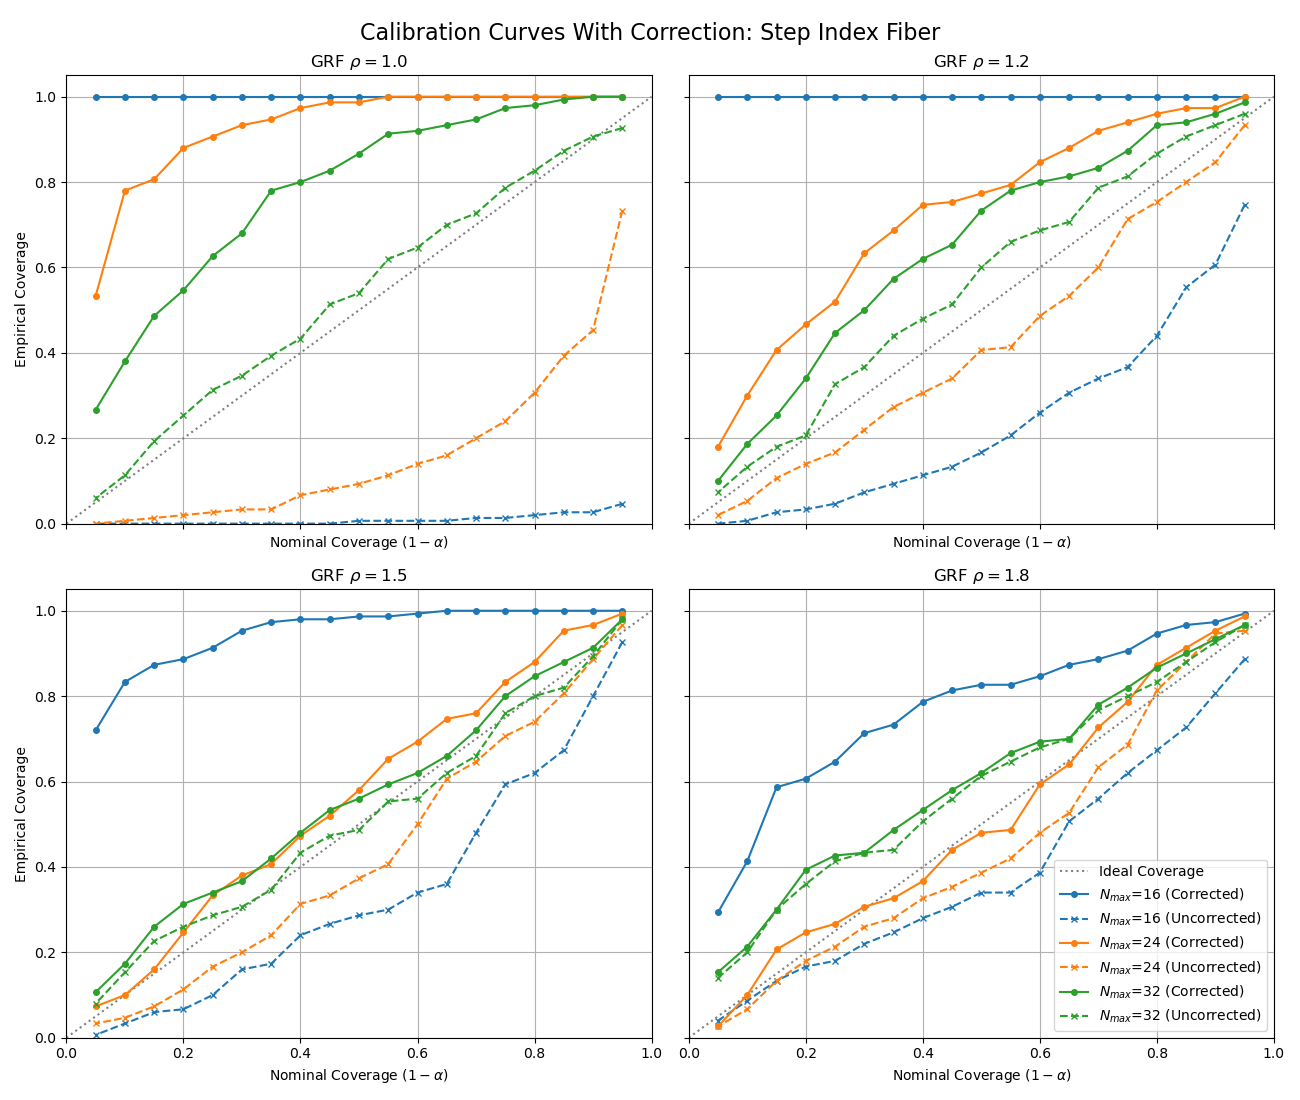
\includegraphics[width=0.97\textwidth]{images/step_index_calibration.png}
  \caption{Calibration curves with (solid) and without (dashed) spectral correction factors across data of varying GRF smoothness parameters for the step-index fiber Hamiltonian. Calibration is performed for three models that act on data at different spectral truncations of the full resolution $N = 64$ data.}
  \label{fig:step_index_calibration}
\end{figure}

\begin{figure}
  \centering 
  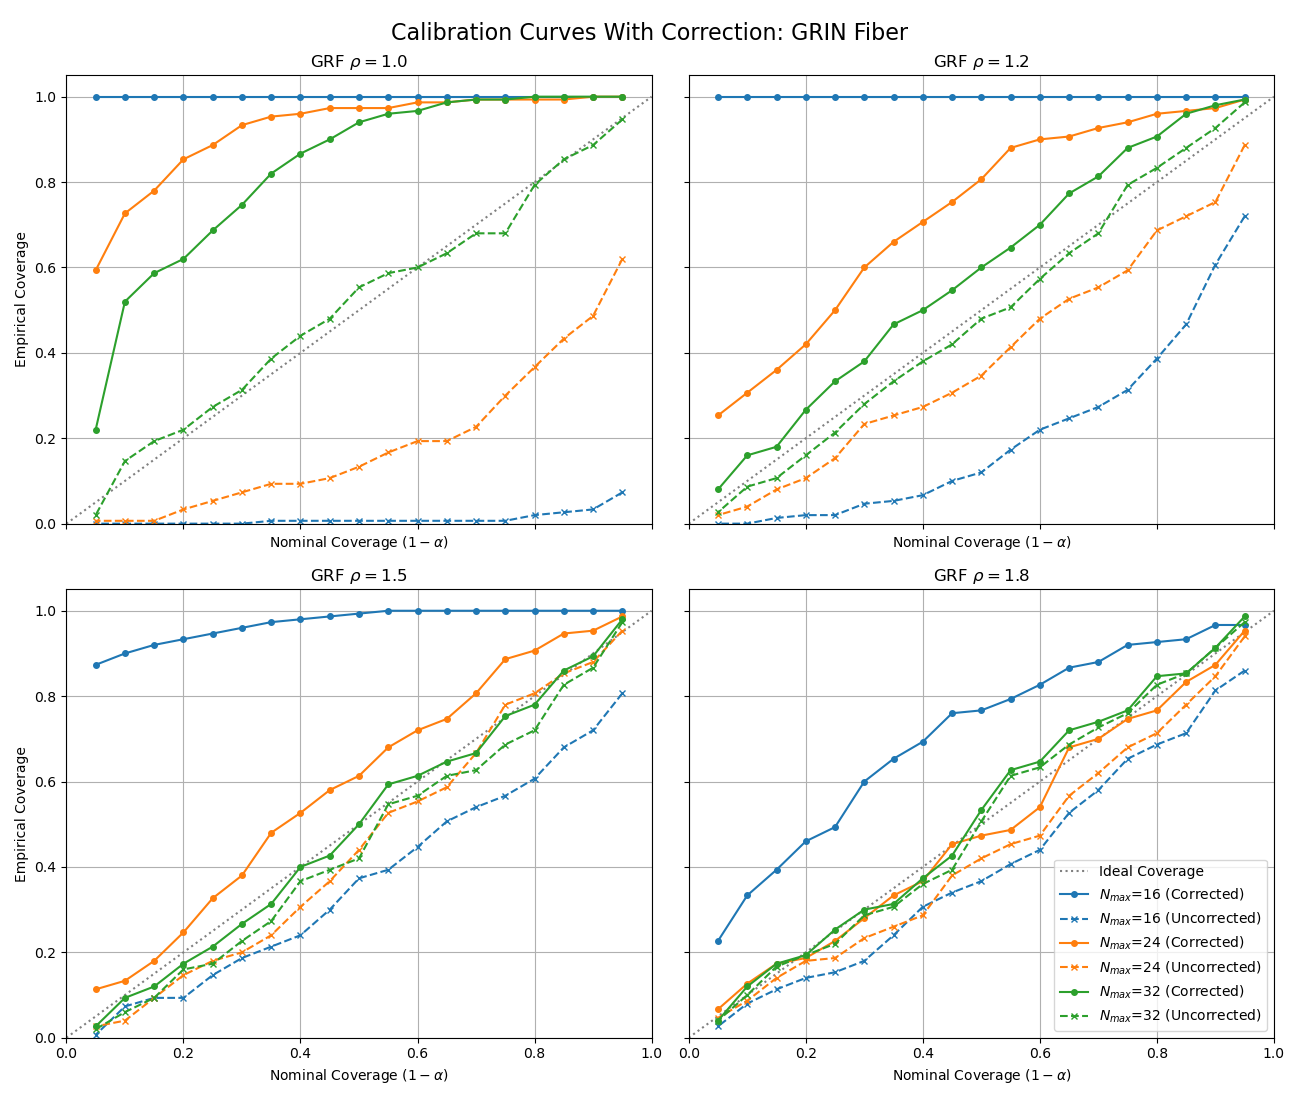
\includegraphics[width=0.97\textwidth]{images/grin_fiber_calibration.png}
  \caption{Calibration curves with (solid) and without (dashed) spectral correction factors across data of varying GRF smoothness parameters for the GRIN fiber Hamiltonian. Calibration is performed for three models that act on data at different spectral truncations of the full resolution $N = 64$ data.}
  \label{fig:grin_calibration}
\end{figure}

Several notable features become apparent from these figures. We first focus on the insights to glean from studying a fixed GRF, such as the case of $\rho=1.2$. First, we notice that, without correction, the models fail to achieve coverage and are consistently underneath the desired calibration curve. After correction, however, all curves achieve coverage at the potential expense of being conservative and overcovering in certain cases. We additionally notice that, as more of the complete spectrum is made visible for training, the uncorrected curves approach the optimal calibration. This is expected as the correction margin is only required to account for unseen modes in the data. In this vein, as the $\rho$ GRF parameter increases, the resulting fields become smoother, thus decreasing the magnitude of the higher, unseen modes in such cases. We, therefore, see that the uncorrected curves get closer to the desired calibration. We additionally notice that, as the correction term is $\propto || \ket{\psi} ||^{2}_{\mathcal{H}^{s}}$, the increasing $\rho$ too is reflected in the correction margin, where the correction desirably decreases as the functions get smoother. This can be seen from the decreasing distance between the uncorrected and corrected calibration curves as $\rho$ increases. Similarly, we notice that the correction margins decrease with increasing $N_{\max}$. This reflects that, as more of the spectrum is observed, there are less unobserved modes that need to be accounted for. Mathematically, this effect emerges from the decay factor $N_{\max}^{-2\nu}$ of the margin. 

% Finally, we notice the aforementioned sensitivity of calibration to the choice of $N_{\mathrm{eff}}$: for sufficiently high choices, coverage is achieved for all levels of truncation at the expense of overly conservative regions. Practically, therefore, this motivates aiming to recover a larger spectrum and to define the margin as tightly as possible from domain knowledge of the nature of the quantum channel. 

% Additional experiments on calibration are presented in \Cref{section:addn_cal}, where we demonstrate the consistency of the findings discussed across different choices of the Hamiltonian.

\subsubsection{Spectral Calibration Across PDEs}\label{section:addn_coverage}

\begin{figure}
  \centering 
  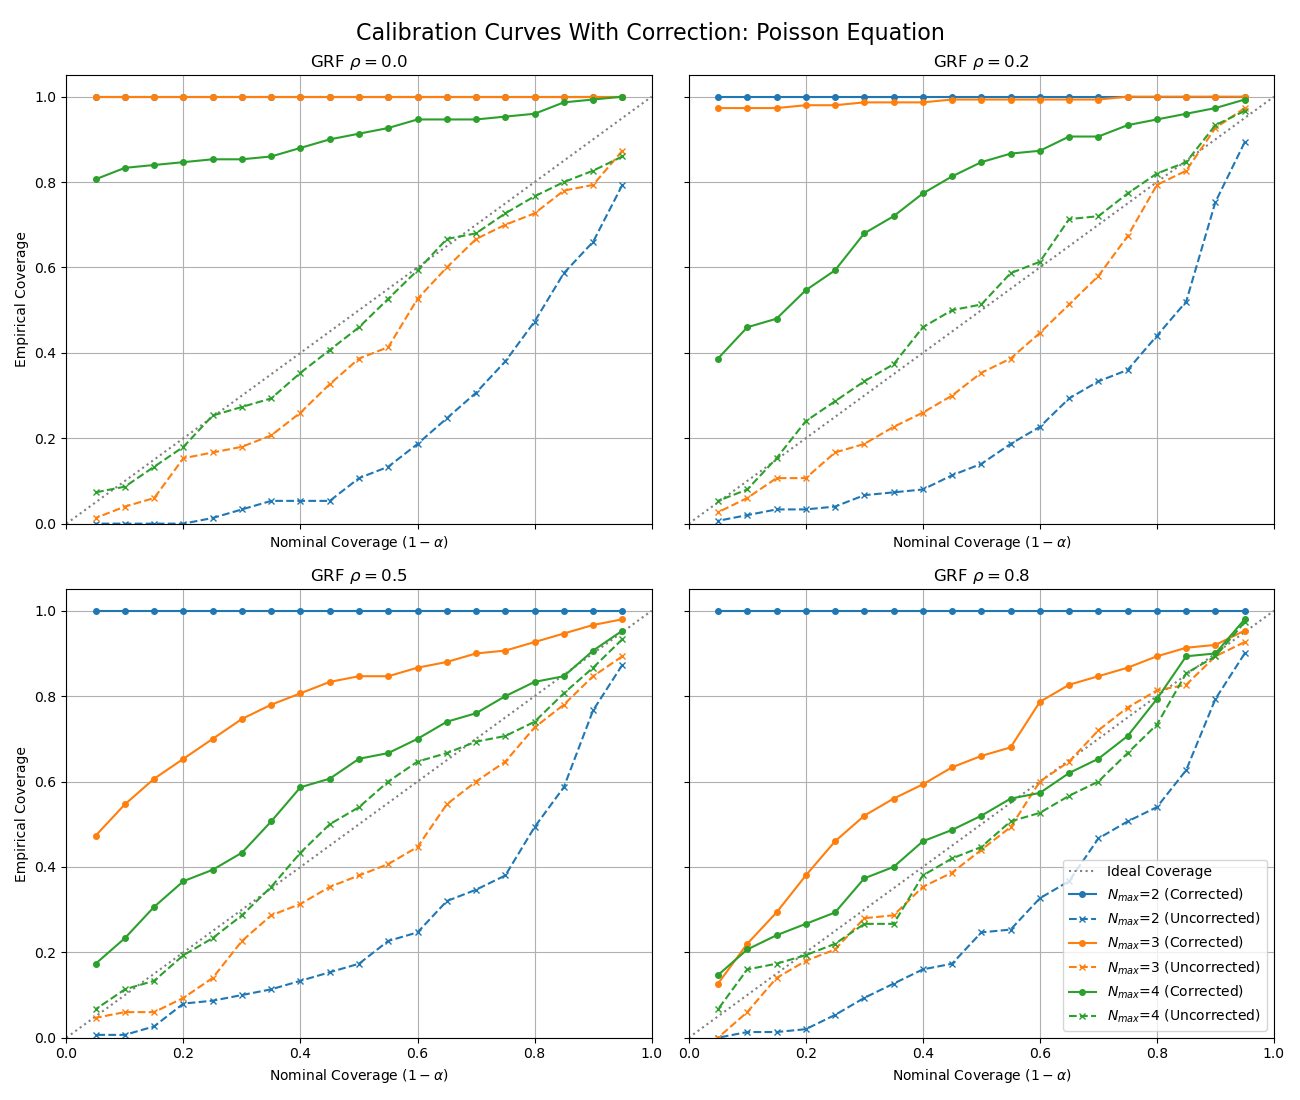
\includegraphics[width=0.97\textwidth]{images/poisson_calibration.png}
  \caption{Calibration curves with spectral correction factors across data of varying GRF smoothness parameters for the Poisson equation. Calibration is performed for three models that act on data at different spectral truncations of the full resolution $N = 64$ data.}
  \label{fig:calibration_poisson}
\end{figure}

As discussed, the calibration procedure presented herein is generally applicable to any PDEs for which a non-trivial bound in the manner of \Cref{lemma:wavefunc_bound} can be expressed. We, therefore, here demonstrate such calibration across two distinct PDE settings, namely the 2D Poisson and 2D heat equations. The 2D Poisson equation is given by
% \begin{equation}
    $\Delta u(x) = f(x)$,
% \end{equation}
where $u : \mathbb{T}^{2}\rightarrow\mathbb{R}$ is the scalar field of interest and $f : \mathbb{T}^{2}\rightarrow\mathbb{R}$ the source field. In this setting, we wish to learn the solution operator $\mathcal{G} : f\to u$.

The heat equation is given by
% \begin{equation}
    $\partial_{t} u = \nu \Delta u,$
% \end{equation}
where now $u : \mathbb{T}^{2}\times[0,T]\rightarrow\mathbb{R}$ is a spatiotemporal field. We, therefore, consider a fixed time $T$ for its evolution, by which the solution operator of interest is purely between the spatial fields $u(\cdot, 0)$ and $u(\cdot, T)$. For each PDE, a dataset of 300 i.i.d. training data points was generated with an additional 150 points used for calibration and 150 for testing coverage. 

% The vorticity equation, in contrast, models the rotational movement of a fluid field. While in general a vector field, if restricted to a 2D fluid field where the velocities are purely in the plane, the vorticity can be expressed purely along the $z$ axis, thereby allowing for a scalar field representation. The 2D vorticity equation is given by
% \begin{equation}
% \begin{aligned}
% \partial_{t} w(x,t) + u(x,t) \cdot \nabla w(x,t) 
%   = \nu \,\Delta w(x,t) + f(x),
%   \quad&x\in\mathbb{T}^2,\; t\in(0,T],\\
% \nabla \cdot u(x,t) = 0, 
%   \quad& x\in\mathbb{T}^2,\; t\in[0,T],\\
% w(x,0) = w_0(x),
%   \quad& x\in\mathbb{T}^2,
% \end{aligned}
% \end{equation}
% where $w : \mathbb{T}^{2}\times[0,T]\rightarrow\mathbb{R}$ is the vorticity, $u : \mathbb{T}^{2}\times[0,T]\rightarrow\mathbb{R}^{2}$ is the underlying fluid flow field, related to the vorticity by $w = \nabla\times u$, $\nu\in\mathbb{R}$ is the fluid viscosity, $f : \mathbb{T}^{2}\rightarrow\mathbb{R}$ the forcing field. Note that, in solving the vorticity PDE, we consider a fixed end time $T$, by which the solution operator of interest is purely between the spatial fields $f$ and $u(\cdot, T)$. To then obtain the corresponding solutions $u_i$, the Dedalus spectral solver \cite{burns2020dedalus} was employed, from which we obtained the full resolution final spectral pairs $(f^{(i)}, \vec{u}^{(i)})$, both resolved to $256\times256$ modes. For each PDE, a complete dataset of 1000 i.i.d. test data points was generated with 500 for calibration and the remaining 500 for testing coverage. 

\begin{figure}
  \centering 
  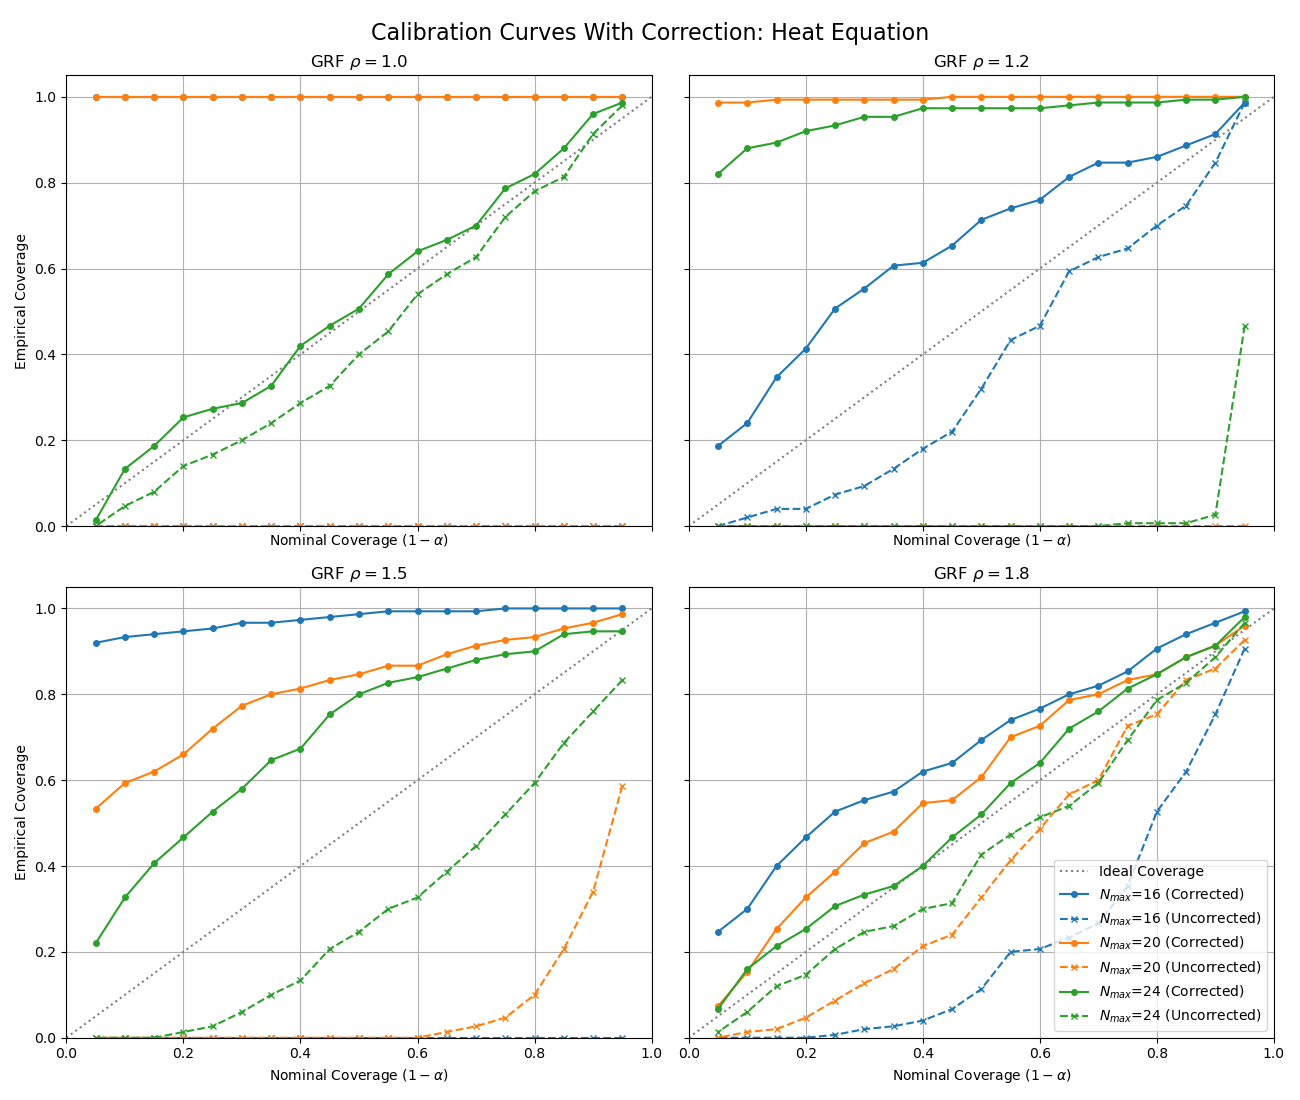
\includegraphics[width=0.97\textwidth]{images/heat_equation_calibration.png}
  \caption{Calibration curves with spectral correction factors across data of varying GRF smoothness parameters for the heat equation. Calibration is performed for three models that act on data at different spectral truncations of the full resolution $N = 64$ data.}
  \label{fig:calibration_heat}
\end{figure}

We once again provide bounds by which we can invoke the results of \Cref{thm:func_cov}. The statement of the Poisson solution bound follows from \Cref{corollary:elliptic_coverage}. We here, however, require the explicit value of $C$ and, thus, provide a full derivation of this bound in \Cref{section:func_bounds}.

\begin{remark}\label{remark:poisson_bound}
    For any zero-mean $u, f\in\mathcal{H}^{s}(\mathbb{T}^{d})$, i.e. $\int_{\mathbb{T}^{d}} u(x)\, dx = \int_{\mathbb{T}^{d}} f(x)\, dx = 0$, for which $\Delta u = f$, $|| u ||^{2}_{\mathcal{H}^{s}(\mathbb{T}^{d})} \le 4 || f ||^{2}_{\mathcal{H}^{s-2}(\mathbb{T}^{d})}$.
\end{remark}

\begin{remark}\label{remark:heat_equation_bound}
    For $u(\cdot, 0)\in\mathcal{H}^{s}(\mathbb{T}^{d})$ such that $\partial_{t} u = \nu \Delta u$, $|| u(\cdot, T) ||^{2}_{\mathcal{H}^{s}(\mathbb{T}^{d})} \le || u(\cdot, 0) ||^{2}_{\mathcal{H}^{s}(\mathbb{T}^{d})}$.
\end{remark}

Using these bounds, we obtain the results shown in \Cref{fig:calibration_poisson} and \Cref{fig:calibration_heat}, where we consider calibration again under different observed spectral truncations across varying smoothness parameters of the GRF. As seen in \Cref{section:wavefunc_coverage}, while all truncations of the spectrum achieve coverage after correction, those with shorter spectral truncations are more sensitive to changes to the correction factor and, hence, result in great conservatism. Additionally, we see as $\rho$ and $N_{\max}$ increase, all curves converge to being calibrated; this is intuitively expected again as the resulting functions are increasingly smooth with increasing $\rho$ and, hence, the need for a correction margin decreases, since the higher order modes decay to 0.

\subsection{Robust State Discrimination}\label{section:state_disc_exp}
We now demonstrate the improvement in using the resulting robust formulation over the nominal formulation as formulated in \Cref{section:spec_op_cal}. We specifically wish to compare the robust formulation against the corresponding nominal approach, where the predicted $\widehat{\mathcal{G}}(\ket{\gamma^{(b)}})$ is simply assumed to be well-specified with the decision appropriately defined using said prediction using the setup described in \Cref{section:exp_setup}. Towards this end, we conduct a hypothesis test on independent trials on 30 test samples sampled as per \Cref{section:exp_setup} using paired t-tests to test
\begin{equation*}
    H_{0} : I_{A;B}(\phi_{\mathrm{rob}}^{*}, g) = I_{A;B}(\phi_{\mathrm{nom}}^{*}, g)
    \qquad
    H_{A} : I_{A;B}(\phi_{\mathrm{rob}}^{*}, g) > I_{A;B}(\phi_{\mathrm{nom}}^{*}, g)
\end{equation*}
where $\phi_{\mathrm{rob}}^{*}$ is as defined in \Cref{eqn:rob_mutual_info} and $\phi_{\mathrm{nom}}^{*} := \argmax_{\phi\in[0,2\pi)^{M}} I_{A;B}(\phi, \widehat{g})$. We similarly run these hypothesis tests against the baseline PGM measurement scheme, denoted $\phi_{\mathrm{PGM}}$. We repeat this procedure across a number of parameter choices, namely for the GRF smoothness parameter $\rho$, the number of GUS states $M$, and the spectral truncation $N_{\max}$. Uncertainty regions for $G$, and subsequently $g$, were defined as per \Cref{section:function_prop} with the corrected calibration quantiles computed per \Cref{section:coverage_guar_exp}; in particular, regions were defined using $\alpha = 0.10$. Notably, while coverage guarantees for $G$ were proven with regions having a radius of $\sqrt{3} M (2\widehat{q}_{\nu}^{*} + (\widehat{q}_{\nu}^{*})^{2})^{1/2}$, we found this to be highly conservative and for $\widehat{q}_{\nu}^{*}$ to suffice as the radius for the $G$ prediction region; future work may seek to theoretically characterize the settings in which this reduced radius suffices for coverage. 

\begin{table*}[t]
\centering
\caption{Mutual informations for PGM, nominal, and robust measurement schemes across varying GRF smoothness parameters $\rho$, GUS state sizes $M$, and spectral truncations $N_{\max}$. Results are presented over 30 i.i.d. test samples, with the $I(\phi)$ columns indicating the average across samples and $H : I(\phi^{(\mathrm{A})}) > I(\phi^{(\mathrm{B})})$ the p-value of the paired t-test of $I(\phi^{(\mathrm{A})}) > I(\phi^{(\mathrm{B})})$.}
\label{tab:rob_opt_comparison}
\resizebox{\textwidth}{!}{
\begin{tabular}{ccc | ccccc | ccccc}
\toprule
 & & & \multicolumn{5}{c}{\textbf{Step-Index Fiber}} & \multicolumn{5}{c}{\textbf{GRIN Fiber}} \\
\cmidrule(lr){4-8} \cmidrule(lr){9-13}
 {$\rho$} & {M} & {$N_{\max}$} & {$I(\phi^{(\mathrm{PGM})})$} & {$I(\phi^{(\mathrm{nom})})$} & {$I(\phi^{(\mathrm{rob})})$} & {$H : I(\phi^{(\mathrm{rob})}) > I(\phi^{(\mathrm{PGM})})$} & {$H : I(\phi^{(\mathrm{rob})}) > I(\phi^{(\mathrm{nom})})$} & {$I(\phi^{(\mathrm{PGM})})$} & {$I(\phi^{(\mathrm{nom})})$} & {$I(\phi^{(\mathrm{rob})})$} & {$H : I(\phi^{(\mathrm{rob})}) > I(\phi^{(\mathrm{PGM})})$} & {$H : I(\phi^{(\mathrm{rob})}) > I(\phi^{(\mathrm{nom})})$} \\
\midrule
1.5 & 3 & 32 & 0.2245 & 0.2613 & \textbf{0.2634} & $< 0.001$ & $< 0.001$ & 0.2157 & 0.2507 & \textbf{0.2526} & $< 0.001$ & $< 0.001$ \\
1.5 & 3 & 48 & 0.2205 & 0.2532 & \textbf{0.2588} & $< 0.001$ & $< 0.001$ & 0.2159 & 0.2161 & \textbf{0.2476} & $< 0.001$ & $< 0.001$ \\
1.5 & 4 & 32 & 0.2144 & 0.2221 & \textbf{0.2222} & $< 0.001$ & 0.268 & 0.2134 & 0.2206 & \textbf{0.2211} & $< 0.001$ & 0.002 \\
1.5 & 4 & 48 & 0.2139 & 0.2203 & \textbf{0.2212} & $< 0.001$ & $< 0.001$ & 0.2127 & 0.2156 & \textbf{0.2160} & $< 0.001$ & 0.093 \\
1.8 & 3 & 32 & 0.2150 & 0.2508 & \textbf{0.2518} & $< 0.001$ & $< 0.001$ & 0.2160 & 0.2529 & \textbf{0.2536} & $< 0.001$ & $< 0.001$ \\
1.8 & 3 & 48 & 0.2205 & 0.2279 & \textbf{0.2532} & $< 0.001$ & $< 0.001$ & 0.2176 & 0.2264 & \textbf{0.2522} & $< 0.001$ & $< 0.001$ \\
1.8 & 4 & 32 & 0.2132 & 0.2206 & \textbf{0.2213} & $< 0.001$ & $< 0.001$ & 0.2187 & 0.2264 & \textbf{0.2271} & $< 0.001$ & $< 0.001$ \\
1.8 & 4 & 48 & 0.2157 & 0.2170 & \textbf{0.2204} & $< 0.001$ & $< 0.001$ & 0.2095 & 0.2118 & \textbf{0.2149} & $< 0.001$ & $< 0.001$ \\
\bottomrule
\end{tabular}}
\end{table*}

The results are presented in \Cref{tab:rob_opt_comparison}. From this, we see that across a diverse collection of problem settings, robust state discrimination significantly outperforms both the baseline PGM and nominal measurement schemes. Notably, holding $\rho$ and $M$ constant, the magnitude of the improvement resulting from robustness generally increases for higher $N_{\max}$. This is a reflection of the result demonstrated in \Cref{lemma:subopt_gap}, namely that the suboptimality bound grows with the conservatism of the prediction region. As discussed in \Cref{section:wavefunc_coverage}, this conservatism is reduced as the quantile correction factor decays, which occurs with the observation of a larger spectral truncation or with increasing smoothness of the underlying functions. Hence, the greater improvement with higher $N_{\max}$ reflects reduced conservatism of the prediction regions. By the same token, the correction factor is reduced in considering a higher $\rho$ for a fixed $M$ and $N_{\max}$, which similarly translates to a greater magnitude of improvement from considering the robust formulation over the nominal or PGM schemes. 

\section{Discussion}\label{section:discussion}
We have here presented an approach to robust, data-driven quantum state discrimination. This work suggests many avenues of extension both continuing in the direction of quantum algorithms and for generalizing the presented method. As discussed, the results presented herein were particular to single particle evolution of a quantum system; quantum communications protocols, however, often leverage lasers with indefinite particle counts. Handling this case would require nontrivial generalizations to the operator learning framework and score definition to work over more general Fock spaces. Similarly, extending the experiments to consider mixed-state density operators and corresponding channels with non-unitary evolution would be of interest. Finally, this framework of robust functionals acting on predictions from operators can be leveraged more broadly, such as in maximal collection problems downstream of Hilbert-space kriging \cite{menafoglio2016kriging,hristopulos2020random, carnevale2021system,vianna2019set,boubrima2017optimal,kessler1998detecting}. Towards this end, we include a preliminary result in \Cref{section:lin_robust} demonstrating that robustness does \textit{not} result in improved decision-making if the downstream functional has certain structural properties; future works should focus on uncovering cases where a separation can be demonstrated.

\newpage
\bibliographystyle{siamplain}
\bibliography{references}

\newpage
\appendix
\section{Explicit Mutual Information Expression}\label{section:explicit_mi}
We here provide for completeness the explicit form of the mutual information objective. Since $I(A;B) := H(B) - H(B\mid A)$, we derive separately the two terms below:
    \begin{align*}
        &H(B) = \sum_{j=0}^{M-1} \mathcal{P}(B = j) \log(\mathcal{P}(B = j)) \\
        &= \sum_{j=0}^{M-1} \sum_{k=0}^{M-1} \mathcal{P}(A = k) \mathcal{P}(B = j | A = k) \log(\sum_{k=0}^{M-1} \mathcal{P}(A = k) \mathcal{P}(B = j | A = k)) \\
        &= \sum_{j=0}^{M-1} \sum_{k=0}^{M-1} q_k \left| \frac{1}{M} \sum_{s=0}^{M-1} e^{-i\phi_s} g_{s}^{1/2} e^{2\pi i s (k-j) / M} \right|^{2} \log  \left(\sum_{k=0}^{M-1} q_k\left| \frac{1}{M} \sum_{s=0}^{M-1} e^{-i\phi_s} g_{s}^{1/2} e^{2\pi i s (k-j) / M} \right|^{2}\right)
    \end{align*}
    Critically, for $H(B\mid A)$, we can use the fact that $H(X)$ only depends on $\mathrm{Law}(X)$. Under GUS, we have $\mathrm{Law}(B\mid A = k) = \mathrm{Law}(B \mid A=0)$. Therefore, it follows that
    \begin{align*}
        H(B\mid A) 
        &= \sum_{k=0}^{M-1} \mathcal{P}(A = k) H(B | A = k) \\
        &= \sum_{k=0}^{M-1} \mathcal{P}(A = k) H(B | A = 0) \\
        &= H(B | A = 0) \sum_{k=0}^{M-1} \mathcal{P}(A = k) = H(B | A = 0)\\
        H(B | A = 0) &:= \sum_{j=0}^{M-1} \mathcal{P}(B = j\mid A = 0) \log(\mathcal{P}(B = j\mid A = 0)) \\
        &:= \sum_{j=0}^{M-1} \left| \frac{1}{M} \sum_{s=0}^{M-1} e^{-i\phi_s} g_{s}^{1/2} e^{-2\pi i j s / M} \right|^{2} \log\left(\left| \frac{1}{M} \sum_{s=0}^{M-1} e^{-i\phi_s} g_{s}^{1/2} e^{-2\pi i j s / M} \right|^{2}\right) 
    \end{align*}

\section{Suboptimality Gap Lemma}\label{section:suboptimalty_gap}
We provide the statement of the general suboptimality gap result to which we wish to appeal below for convenience.

\begin{lemma}\label{lemma:cp_subopt}
    (Lemma 3.1 of \cite{patel2024conformal}) Consider any $f(w, c)$ that is $L$-Lipschitz in $c$ under the metric $d$ for any fixed $w$. Assume further that $\mathcal{P}_{X,C}(C \in \mathcal{U}(X)) \ge 1 - \alpha$. Then, 
    \begin{equation}
        \mathcal{P}_{X,C}\left(0\le \Delta(X, C) \le L \max_{\widehat{c}\in\mathcal{U}(X)}d(C, \widehat{c})\right) \ge 1 - \alpha,
    \end{equation}
    where $\Delta(x, c) := \min_{w} \max_{\widehat{c}\in\mathcal{U}(x)} f(w, \widehat{c}) - \min_{w} f(w, c)$.
\end{lemma}

\begin{lemma}
    Let $\Delta_{\mathrm{MI}}(\vec{\gamma}^{(b)}, g)$ be as defined in \Cref{eqn:mi_subopt}. Assume that $\mathcal{P}_{\vec{\gamma}^{(b)}, g}(|| g - \widehat{g} ||^{2}_{2}\le\widehat{q})\ge 1-\alpha$. Further, suppose \Cref{assup:min_prob} is satisfied. Then, for a constant $L < \infty$,
    \begin{equation}
        \mathcal{P}_{\vec{\gamma}^{(b)}, g}(\Delta_{\mathrm{MI}}(\vec{\gamma}^{(b)}, g) \le L \sqrt{\widehat{q}})\ge 1-\alpha.
    \end{equation}
\end{lemma}

\begin{proof}
    To appeal to \Cref{lemma:cp_subopt}, we first re-express our suboptimality gap in the min-max form desired, namely as
    \begin{align*}
        \Delta_{\mathrm{MI}}(\vec{\gamma}^{(b)}, g) 
        % &:= \max_{\phi\in[0,2\pi)^{M}} I_{A; B}(\phi, g) - \max_{\phi\in[0,2\pi)^{M}} \min_{\widehat{g}\in\mathcal{C}_{\widehat{q}}(\vec{\gamma}^{(b)})} I_{A; B}(\phi, \widehat{g}) \\
        &= \min_{\phi\in[0,2\pi)^{M}} \max_{\widehat{g}\in\mathcal{C}_{\widehat{q}}(\vec{\gamma}^{(b)})} (-I_{A; B}(\phi, \widehat{g})) - \min_{\phi\in[0,2\pi)^{M}} (-I_{A; B}(\phi, g))
    \end{align*}
    In this re-expressed form, it suffices to demonstrate $-I_{A; B}(\phi, \widehat{g})$ is $L$-Lipschitz in $g$ for any fixed $\phi$. We demonstrate this by first considering a fixed $\phi$, defining the corresponding Lipschitz constant $L(\phi)$, and then considering the supremum over this domain. Since $-I_{A; B}(\phi, g) := H(B\mid A) - H(B) = H(B\mid A = 0) - H(B)$, where the latter equality was discussed in \Cref{section:explicit_mi}, it suffices to demonstrate each of $H(B)$ and $H(B\mid A = 0)$ are Lipschitz in $g$. We do so by first introducing auxiliary variables $p_j$ and $p_{j|0}$, demonstrating that $H(B)$ and $H(B\mid A = 0)$ are respectively Lipschitz in these variables, and concluding by demonstrating the maps $g\to p_j$ and $g\to p_{j|0}$ are Lipschitz.

    To begin, we see $H(B)$ takes the form $\sum_{j} p_j \log(p_j)$, where $p_j := \mathcal{P}(B = j)$. Clearly, $| \partial_{p_j} (p_j \log(p_j)) | = | 1 + \log(p_j) | \le |1 + \log(\epsilon)|$ if $p_j\ge \epsilon > 0$, meaning $H(B)$ is Lipschitz in $p_j$ if $p_j$ is lower bounded. Such a lower bound follows as, under GUS, $\mathcal{P}(B = j\mid A = k) = \mathcal{P}(B = (j - k) \text{ mod } M \mid A = 0)$. By \Cref{assup:min_prob}, we have $\mathcal{P}(B = (j - k) \text{ mod } M \mid A = 0) > 0$. Thus, for any $j$,
    \begin{align*}
        \mathcal{P}(B = j) 
        = \sum_{k=0}^{M-1} \mathcal{P}(B = j | A = k) \mathcal{P}(A = k)
        = \sum_{k=0}^{M-1} q_k \mathcal{P}(B = (j - k) \text{ mod } M \mid A = 0) > 0        
    \end{align*}
    The Lipschitzness of $H(B\mid A = 0) = \sum_{j} \mathcal{P}(B = j\mid A = 0) \log(\mathcal{P}(B = j\mid A = 0))$ follows immediately, since the lower bound on $\mathcal{P}(B = j\mid A = 0)$ exists by \Cref{assup:min_prob}.
    
    To conclude this proof, we simply need to show the maps $g\to p_j$ and $g\to p_{j|0}$ are Lipschitz. Recall that
    \begin{align*}
        p_{j}  := \sum_{k=0}^{M-1} q_k\left| \frac{1}{M} \sum_{s=0}^{M-1} e^{-i\phi_s} g_{s}^{1/2} e^{2\pi i s (k-j) / M} \right|^{2}
        \qquad p_{j|0} := \left| \frac{1}{M} \sum_{s=0}^{M-1} e^{-i\phi_s} g_{s}^{1/2} e^{-2\pi i s j / M} \right|^{2}
    \end{align*}
    Clearly, it suffices to show the map $g\to p_{j|0}$ is Lipschitz, as $g\to p_j$ is then simply the sum of such functions whose Lipschitzness can be shown identically. We do this explicitly by bounding the gradient as follows, where we denote by $c_{s} := e^{-2\pi i s j / M}$:
    \begin{align*}
        p_{j|0}
        &= \left| \frac{1}{M} \sum_{s=0}^{M-1} c_{s} e^{-i\phi_s} g_{s}^{1/2} \right|^{2} \\
        &= \left( \frac{1}{M} \sum_{s=0}^{M-1} c_{s} e^{-i\phi_s} g_{s}^{1/2} \right) \overline{\left( \frac{1}{M} \sum_{s'=0}^{M-1} c_{s'} e^{-i\phi_{s'}} g_{s'}^{1/2} \right)} \\
        &= \frac{1}{M^{2}} \sum_{s=0}^{M-1} \sum_{s'=0}^{M-1} c_{s} \overline{c_{s'}} e^{-i\phi_s} e^{i\phi_{s'}} g_{s}^{1/2} g_{s'}^{1/2}
    \end{align*}
    We now compute the gradient component-wise:
    \begin{align*}
        \partial_{g_{r}} p_{j|0}
        &= \frac{1}{M^{2}} \sum_{s=0}^{M-1} \sum_{s'=0}^{M-1} \left(c_{s} \overline{c_{s'}} e^{-i\phi_s} e^{i\phi_{s'}} \right) \partial_{g_{r}} (g_{s}^{1/2} g_{s'}^{1/2}) \\
        &= \frac{1}{M^{2}} \sum_{s=0}^{M-1} \sum_{s'=0}^{M-1} \left(c_{s} \overline{c_{s'}} e^{-i\phi_s} e^{i\phi_{s'}} \right) \left(\frac{1}{2} g_{s}^{-1/2} g_{s'}^{1/2} \delta_{sr} + \frac{1}{2} g_{s}^{1/2} g_{s'}^{-1/2} \delta_{s'r}\right) \\
        &= \frac{1}{2 M^{2}} \left( \sum_{s=0}^{M-1} \sum_{s'=0}^{M-1} c_{s} \overline{c_{s'}} e^{-i\phi_s} e^{i\phi_{s'}} g_{s}^{-1/2} g_{s'}^{1/2} \delta_{sr} + \sum_{s=0}^{M-1} \sum_{s'=0}^{M-1} c_{s} \overline{c_{s'}} e^{-i\phi_s} e^{i\phi_{s'}} g_{s}^{1/2} g_{s'}^{-1/2} \delta_{s'r}\right) \\
        &= \frac{1}{2 M^{2}} \left( \sum_{s'=0}^{M-1} \underbrace{c_{r} \overline{c_{s'}} e^{-i\phi_r} e^{i\phi_{s'}}}_{b_{s'}} g_{r}^{-1/2} g_{s'}^{1/2} + \sum_{s=0}^{M-1} \underbrace{c_{s} \overline{c_{r}} e^{-i\phi_s} e^{i\phi_{r}}}_{a_{s}} g_{s}^{1/2} g_{r}^{-1/2} \right)
    \end{align*}    
    Critically, we now recognize that $s'$ is a dummy index and can be replaced with the index $s$. With this relabeling, we notice $\overline{b_{s}} = a_{s}$, from which this expression simplifies to $2 \mathrm{Re}(a_{s})$:
    \begin{align*}
        \partial_{g_{r}} p_{j|0} = \frac{1}{2 M^{2}} \left( \sum_{s=0}^{M-1} 2 \mathrm{Re} (c_{r} \overline{c_{s}} e^{-i\phi_r} e^{i\phi_{s}}) g_{r}^{-1/2} g_{s}^{1/2} \right)
        = \frac{1}{M^{2}} \mathrm{Re} \left( c_{r} e^{-i\phi_r} g_{r}^{-1/2} \sum_{s=0}^{M-1} \overline{c_{s}} e^{i\phi_{s}} g_{s}^{1/2} \right) 
    \end{align*}
    Using this per-component expression, we can bound the gradient simply as
    \begin{align*}
        || \nabla_{g} p_{j|0} ||^{2}
        \le \sup_{g\in\mathcal{C}_{\widehat{q}}(\vec{\gamma}^{(b)})} \underbrace{\sum_{r=0}^{M-1} \left| \frac{1}{M^{2}} \mathrm{Re} \left( c_{r} e^{-i\phi_r} g_{r}^{-1/2} \sum_{s=0}^{M-1} \overline{c_{s}} e^{i\phi_{s}} g_{s}^{1/2} \right) \right|^{2}}_{:= \widehat{L}_{p|0}(\phi, g)}
        =: L_{p|0}(\phi)
    \end{align*}
    Notably, this bound $L_{p|0}(\phi)$ is finite if $g_r > 0$. Recall that $G = \Gamma^{\dagger} \Gamma$ for a collection of linearly \textit{independent} $\{\ket{\gamma_k}\}$. It, therefore, follows that $G\succ 0$, from which we get that $g_r > 0$ for all $r = 0, ..., M-1$, thereby demonstrating $|| \nabla_{g} p_{j|0} ||$ is bounded and, hence, $g\to p_{j|0}$ is Lipschitz.
    
    Thus, since each of $g\to p_j$ and $g\to p_{j|0}$ are Lipschitz and so too are $p_j\to H(B)$ and $p_{j|0}\to H(B\mid A = 0)$, their composition too is Lipschitz in $g$, from which it follows that there exists some constant $L(\phi)$ for which $-I_{A; B}(\phi, g)$ is the Lipschitz constant in $g$ for this fixed $\phi$. Finally, by the explicit gradient bound derived above, we see the maps $\phi\to L_{p|0}(\phi)$ and $\phi\to L_{p}(\phi)$ are continuous. This follows as the bound $\widehat{L}_{p|0}(\phi, g)$ is a continuous function jointly over $\phi$ and $g$, from which it follows that $\sup_{g\in\mathcal{C}_{\widehat{q}}(\vec{\gamma}^{(b)})} \widehat{L}_{p|0}(\phi, g)$ is continuous in $\phi$ as $\mathcal{C}_{\widehat{q}}(\vec{\gamma}^{(b)})$ is compact. This coupled with the fact that $p_j\to H(B)$ and $p_{j|0}\to H(B\mid A = 0)$ too are continuous, implies the full map $\phi\to L(\phi)$ is continuous. Finally, as we are considering a periodic domain $[0, 2\pi)^{M}$, we can consider the supremum identically over the closed \textit{compact} domain $L := \sup_{\phi\in [0, 2\pi]^{M}} L(\phi)$, which must be finite by the extreme value theorem, as $L(\phi)$ is bounded and continuous.
\end{proof}

\begin{proof}
For each stage $t$, define
\[
\phi_t(w)\ :=\ \max_{\vec u^{(t)}\in \mathcal{C}_{N_t;\nu}(\vec a)} J[w,\vec u^{(t)}],
\qquad
w_t^* \in \arg\min_w \phi_t(w).
\]
By Danskin’s theorem, for any $w$ there exists a maximizer $u_t^*(w)\in\mathcal C_{N_t;\nu}(\vec a)$
such that
\[
\nabla \phi_t(w)\ =\ \nabla_w J\!\bigl(w, u_t^*(w)\bigr).
\]
Likewise for stage $t\!-\!1$ with a maximizer $u_{t-1}^*(w)\in\mathcal C_{N_{t-1};\nu}(\vec a)$.
Using the assumed Lipschitz continuity of $\nabla_w J$ in $u$ with constant $G_u$ under $\|\cdot\|_{s-\nu}$,
\[
\bigl\|\nabla\phi_t(w)-\nabla\phi_{t-1}(w)\bigr\|
\ =\
\bigl\|\nabla_w J\!\bigl(w,u_t^*(w)\bigr)-\nabla_w J\!\bigl(w,u_{t-1}^*(w)\bigr)\bigr\|
\ \le\ G_u\,\bigl\|u_t^*(w)-u_{t-1}^*(w)\bigr\|_{s-\nu}.
\]
The sets $\mathcal C_{N_{t-1};\nu}(\vec a)\subseteq \mathcal C_{N_t;\nu}(\vec a)$ are (centered) balls with radii
\[
r_{t-1} = \sqrt{4 \widehat{q}_{N_{t-1};\nu} + B N_{t-1}^{-2\nu}},\qquad
r_{t} = \sqrt{4 \widehat{q}_{N_{t};\nu} + B N_{t}^{-2\nu}},
\]
so we may select maximizers with
\(
\|u_t^*(w)-u_{t-1}^*(w)\|_{s-\nu}\le (r_t-r_{t-1})_+.
\)
Hence
\begin{equation}
\sup_w \bigl\|\nabla\phi_t(w)-\nabla\phi_{t-1}(w)\bigr\|
\ \le\ G_u\,(r_t-r_{t-1})_+ .
\label{eq:grad-gap}
\end{equation}

\paragraph{Drift of minimizers.}
Because each $\phi_t$ is $\mu$-strongly convex in $w$, the standard sensitivity bound for minimizers under gradient perturbations gives
\begin{equation}
\|w_t^*-w_{t-1}^*\|
\ \le\ \frac{1}{\mu}\,\sup_w \bigl\|\nabla\phi_t(w)-\nabla\phi_{t-1}(w)\bigr\|
\ \stackrel{\eqref{eq:grad-gap}}{\le}\ \frac{G_u}{\mu}\,(r_t-r_{t-1})_+ .
\label{eq:drift}
\end{equation}

\paragraph{Per-stage iteration complexity.}
Run gradient descent on $\phi_t$ with step $1/L_w$, initialized at $w_{t-1}^*$. For a $(\mu,L_w)$ function,
\[
\phi_t(w_k)-\phi_t(w_t^*)\ \le\ \Bigl(1-\frac{\mu}{L_w}\Bigr)^{k}\,\frac{L_w}{2}\,\|w_{t-1}^*-w_t^*\|^2.
\]
Stop at the first $k=K_t$ with $\phi_t(w_k)-\phi_t(w_t^*)\le \varepsilon_t$. Solving for $K_t$,
\[
K_t\ \le\ \frac{1}{\bigl|\log(1-\mu/L_w)\bigr|}\,
\log\!\left(\frac{L_w}{2\,\varepsilon_t}\,\|w_{t-1}^*-w_t^*\|^2\right).
\]
Using \eqref{eq:drift} to bound the warm-start distance,
\begin{equation}
K_t\ \le\ \frac{1}{\bigl|\log(1-\mu/L_w)\bigr|}\,
\log\!\left(
\frac{L_w}{2\,\varepsilon_t}\,
\Bigl(\tfrac{G_u}{\mu}\Bigr)^{\!2}\,(r_t-r_{t-1})_+^{2}
\right).
\label{eq:Kt}
\end{equation}

\paragraph{Total cost.}
By definition $\mathcal E^{(t)}=C_{N_t}\,K_t$ and
\(
\mathcal E(\{N_t\})=\sum_{t=1}^T \mathcal E^{(t)}.
\)
Summing \eqref{eq:Kt} over $t$ yields
\[
\mathcal E(\{N_t\})\ \le\
\frac{1}{\bigl|\log(1-\mu/L_w)\bigr|}\,
\sum_{t=1}^{T}
C_{N_t}\;
\log\!\left(
\frac{L_w}{2\,\varepsilon_t}\,
\Bigl(\tfrac{G_u}{\mu}\Bigr)^{\!2}\,(r_t-r_{t-1})_+^{2}
\right).
\]
This is the claimed multi-stage bound (up to the two notational fixes noted above). Finally, the condition $r_T<\varepsilon/L$ is exactly your finite-dimensional coverage guarantee translated through the $L$-Lipschitz continuity of $J$ in $u$, ensuring the terminal stage achieves the target suboptimality budget.
\end{proof}


\newpage
\section{Functional Coverage Guarantee}\label{section:coverage_guarantee}
\begin{theorem}
    Let $(\vec{a}^{(i)}, \{\widehat{u}_n\})\cup (\vec{a}', \{\widehat{u}'_n\})\sim\mathcal{P}(\vec{A}, \{\widehat{U}_n\})$ and $\mathcal{P}(|| \{\widehat{U}_n\} ||^{2}_{\mathcal{H}_s(\mathbb{T}^{d})}\le B) = 1$ for some $B \ge 0$. Further, let $\mathcal{D}_{C} := \{(\vec{a}^{(i)}, \vec{u}^{(i)})\}$. Let $\alpha\in(0,1)$ and $\widehat{q}_{\nu}$ be the $\ceil{(N_{C}+1)(1-\alpha)}/N_{C}$ quantile of \Cref{eqn:score_func} over $\mathcal{D}_{C}$ for a fixed $\mathcal{G}$ and $\nu\in\{1,...,s\}$. Then
    \begin{equation}
        \mathcal{P}_{\vec{A}', \{\widehat{U}'_n\}}\left(\sum_{n\in\mathbb{Z}^{d}} (1 + || n ||_{2}^{2})^{s-\nu} ([\mathcal{G}(\vec{A}')]_{n} - U'_{n})^{2}
        \le \widehat{q}_{\nu} + B N_{\max}^{-2\nu} \right) \ge 1-\alpha.
    \end{equation}
\end{theorem}
\begin{proof}
    We consider the event of interest conditionally on $s_{\nu}(\vec{a}', \{\widehat{u}'_n\})\le\widehat{q}_{\nu}$. Then:
    \begin{align*}
        &\sum_{n\in\mathbb{Z}^{d}} (1 + || n ||_{2}^{2})^{s-\nu} ([\mathcal{G}(\vec{a}')]_{n} - u'_{n})^{2}  \\
        &= \underbrace{ \sum_{n\in\mathbb{Z}^{d} : | n |_{\infty} \le N_{\max}} (1 + || n ||_{2}^{2})^{s-\nu} ([\mathcal{G}(\vec{a}')]_{n} - u'_{n})^{2}}_{\mathcal{E}_{\le N_{\max}}} + \underbrace{ \sum_{n\in\mathbb{Z}^{d} : | n |_{\infty} > N_{\max}} (1 + || n ||_{2}^{2})^{s-\nu} (u'_{n})^{2} }_{\mathcal{E}_{> N_{\max}}}
    \end{align*}
    We now demonstrate how each of the above two terms can be bounded. For the former, the result immediately follows in noting that $\mathcal{E}_{\le N_{\max}}$ is precisely $s_{\nu}(\vec{a}', \vec{u}')$, from which we have $\mathcal{E}_{\le N_{\max}}\le\widehat{q}_{\nu}$ directly by assumption on $(\vec{a}', \vec{u}')$. For the latter, we appeal to standard techniques for Fourier truncation analysis as follows
    \begin{align*}
        \sum_{n\in\mathbb{Z}^{d} : | n |_{\infty} > N_{\max}} & (1 + || n ||_{2}^{2})^{s-\nu} (u'_{n})^{2} 
        =  \sum_{n\in\mathbb{Z}^{d} : | n |_{\infty} > N_{\max}} \frac{(1 + || n ||_{2}^{2})^{s}}{(1 + || n ||_{2}^{2})^{\nu}} (u'_{n})^{2}  \\
        &\le \frac{1}{(1 + N_{\max}^{2})^{\nu}}  \sum_{n\in\mathbb{Z}^{d} : | n |_{\infty} > N_{\max}} (1 + || n ||_{2}^{2})^{s} (u'_{n})^{2}
        \le B N_{\max}^{-2\nu}.
    \end{align*}
    We conclude by noting that $\mathcal{P}_{\vec{A}', \{\widehat{U}'_n\}}(s_{\nu}(\vec{A}', \{\widehat{U}'_n\})\le\widehat{q}_{\nu}) \ge 1 - \alpha$ from standard results of conformal prediction, completing the proof.  
\end{proof}

\section{Elliptic Regularity Theory}\label{section:regularity_theory}
We here state the relevant bounds provided by classical elliptic regularity theory for reference from which \Cref{corollary:elliptic_coverage} immediately follows. We present below a special case of the general statement presented in \cite{Sturm_EllipticPDE_2017}, where we consider scalar fields (i.e. restrict operators to be of rank $m=1$) defined over $\mathbb{T}^{d}$.

% \begin{theorem}
%     (Theorem 5, Chapter 6 of \cite{evans2022partial}) Let $s$ be a nonnegative integer, and assume $a^{ij}, b^{i}, c \in \mathcal{C}^{s+1}(\overline{\mathbb{T}^{d}}) \quad (i, j = 1, \ldots, n)$ and $f \in \mathcal{H}^{s}(\mathbb{T}^{d})$. Suppose that $u \in \mathcal{H}^{1}_{0}(\mathbb{T}^{d})$ is a weak solution of the boundary-value problem
%     \begin{align}
%         % \begin{cases}
%             Lu = f \quad x\in\mathbb{T}^{d}
%             \qquad u = 0 \quad x\in\partial\mathbb{T}^{d}.
%         % \end{cases}
%     \end{align}
%     Assume finally $\partial \mathbb{T}^{d} \text{ is } \mathcal{C}^{s+2}.$
%     Then $u \in \mathcal{H}^{s+2}(\mathbb{T}^{d}),$ and we have the estimate
%     \begin{align}\label{eqn:sobolev_bound}
%         \|u\|_{\mathcal{H}^{s+2}(\mathbb{T}^{d})} \leq C \left( \|f\|_{\mathcal{H}^{s}(\mathbb{T}^{d})} + \|u\|_{L^{2}(\mathbb{T}^{d})} \right),
%     \end{align}
%     the constant $C$ depending only on $s$, $\mathbb{T}^{d}$ and the coefficients of $L$. If $u$ is further the unique solution of \Cref{eqn:sobolev_bound_setup}, then estimate \Cref{eqn:sobolev_bound} simplifies to read
%     \begin{align}
%         \|u\|_{\mathcal{H}^{s+2}(\mathbb{T}^{d})} \leq C \|f\|_{\mathcal{H}^{s}(\mathbb{T}^{d})}.
%     \end{align}
% \end{theorem}

\begin{theorem}
     (Theorem 6 of \cite{Sturm_EllipticPDE_2017}) Let $L$ be an elliptic operator of order $\ell$ on $\mathbb{T}^{d}$ such that $Lu = f$. Then, there exists $C(L, s)$ such that for $u \in \mathcal{H}^{s+\ell}(\mathbb{T}^{d}) \cap \mathrm{Ker}(L)^{\perp}$, $f \in \mathcal{H}^{s}(\mathbb{T}^{d})$ and
     \begin{equation}
         \|u\|_{\mathcal{H}^{s+\ell}(\mathbb{T}^{d})} \leq C(L, s) \|f\|_{\mathcal{H}^{s}(\mathbb{T}^{d})}
     \end{equation}
\end{theorem}

\section{Gram Matrix Uncertainty Propagation Derivation}\label{section:func_prop_der}
We now derive a probabilistic upper bound on the difference between the estimated and true Gram matrices. Note that, by $\mathcal{P}_{\vec{\gamma}^{(b)}, \ket{\gamma^{(a)}}}(|| \mathcal{G}(\vec{\gamma}^{(b)}) - \ket{\gamma^{(a)}} ||^{2}_{\mathcal{H}^{s-\nu}(\mathbb{T}^{d})} \le \widehat{q}_{\nu}^{*}) \ge 1-\alpha$, it follows that, with the same probabilistic guarantee, $\exists \Delta$ such that $|| \Delta ||^{2}_{\mathcal{H}^{s-\nu}(\mathbb{T}^{d})}\le\widehat{q}_{\nu}^{*}$ and $\mathcal{G}(\vec{\gamma}^{(b)}) = \ket{\gamma^{(a)}} + \Delta$. With this, the desired matrix bound can be immediately established by bounding the difference in each entry as follows, where we use the fact that the true states are normalized in $\mathcal{L}^2$:
\begin{align*}
    || G - \widehat{G} ||^{2}_{F}
    &:= \sum_{\ell, k = 0}^{M-1} | G_{\ell, k} - \widehat{G}_{\ell, k} |^{2} \\
    &:= \sum_{\ell, k = 0}^{M-1} \left| \braket{ \mathcal{G}(\vec{\gamma}^{(b)}_{\ell}) | \mathcal{G}(\vec{\gamma}^{(b)}_{k})} - \braket{ \gamma^{(a)}_{\ell} | \gamma^{(a)}_{k}} \right|^{2} \\
    &= \sum_{\ell, k = 0}^{M-1} \left| \braket{ \gamma_{\ell}^{(a)} + \Delta_{\ell} | \gamma_{k}^{(a)} + \Delta_{k} } - \braket{ \gamma^{(a)}_{\ell} | \gamma^{(a)}_{k}} \right|^{2} \\
    &= \sum_{\ell, k = 0}^{M-1} \left| 
    \braket{ \gamma_{\ell}^{(a)} | \gamma_{k}^{(a)} } 
    + \braket{ \gamma_{\ell}^{(a)} | \Delta_{k} } 
    + \braket{ \Delta_{\ell} | \gamma_{k}^{(a)} } 
    + \braket{ \Delta_{\ell} | \Delta_{k} } 
    - \braket{ \gamma^{(a)}_{\ell} | \gamma^{(a)}_{k}} \right|^{2} \\
    &\le 3 \sum_{\ell, k = 0}^{M-1} 
    \left(| \braket{ \gamma_{\ell}^{(a)} | \Delta_{k} } |^{2}
    + | \braket{ \Delta_{\ell} | \gamma_{k}^{(a)} } |^{2}
    + | \braket{ \Delta_{\ell} | \Delta_{k} } |^{2}\right) \\
    &\le 3 \sum_{\ell, k = 0}^{M-1} \left(
    || \gamma_{\ell}^{(a)} ||^{2}_{\mathcal{L}^{2}} || \Delta_{k} ||^{2}_{\mathcal{L}^{2}}
    + || \Delta_{\ell} ||^{2}_{\mathcal{L}^{2}} || \gamma_{k}^{(a)} ||^{2}_{\mathcal{L}^{2}}
    + || \Delta_{\ell} ||^{2}_{\mathcal{L}^{2}} || \Delta_{k} ||^{2}_{\mathcal{L}^{2}} \right) \\
    &= 3 \sum_{\ell, k = 0}^{M-1} \left( || \Delta_{k} ||^{2}_{\mathcal{L}^{2}} + || \Delta_{\ell} ||^{2}_{\mathcal{L}^{2}}  + || \Delta_{\ell} ||^{2}_{\mathcal{L}^{2}} || \Delta_{k} ||^{2}_{\mathcal{L}^{2}} \right) \\
    &\le 3 \sum_{\ell, k = 0}^{M-1} \left( || \Delta_{k} ||^{2}_{\mathcal{H}^{s-\nu}} + || \Delta_{\ell} ||^{2}_{\mathcal{H}^{s-\nu}}  + || \Delta_{\ell} ||^{2}_{\mathcal{H}^{s-\nu}} || \Delta_{k} ||^{2}_{\mathcal{H}^{s-\nu}} \right) \\
    &\le 3 \sum_{\ell, k = 0}^{M-1} (2\widehat{q}_{\nu}^{*} + (\widehat{q}_{\nu}^{*})^{2})
    = 3 M^2 (2\widehat{q}_{\nu}^{*} + (\widehat{q}_{\nu}^{*})^{2})
\end{align*}

Since $\phi_t$ is $L_t$-smooth, the descent lemma gives, for any stepsize $\eta_t\in(0,1/L_t]$,
\[
\phi_t\bigl(w^{(k+1)}\bigr)
\;\le\;
\phi_t\bigl(w^{(k)}\bigr)
-\eta_t\Bigl(1-\tfrac{L_t\eta_t}{2}\Bigr)\,\|\nabla\phi_t(w^{(k)})\|^2.
\]
With $\eta_t=1/L_t$ this simplifies to
\[
\phi_t\bigl(w^{(k+1)}\bigr)
\;\le\;
\phi_t\bigl(w^{(k)}\bigr)
-\frac{1}{2L_t}\,\|\nabla\phi_t(w^{(k)})\|^2.
\]
Moreover, $\mu$-strong convexity implies the Polyak–Łojasiewicz (PL) inequality
\[
\|\nabla\phi_t(w)\|^2 \;\ge\; 2\mu\bigl(\phi_t(w)-\phi_t(w^\star)\bigr),
\quad\text{where } w^\star:=w^\star(N_t).
\]
Combining the two displays yields the \emph{gap contraction}
\[
\phi_t\bigl(w^{(k+1)}\bigr)-\phi_t(w^\star)
\;\le\;
\Bigl(1-\tfrac{\mu}{L_t}\Bigr)\,\bigl(\phi_t(w^{(k)})-\phi_t(w^\star)\bigr).
\]
By induction,
\[
\phi_t\bigl(w^{(k)}\bigr)-\phi_t(w^\star)
\;\le\;
\Bigl(1-\tfrac{\mu}{L_t}\Bigr)^k
\bigl(\phi_t(w^{(0)})-\phi_t(w^\star)\bigr),
\]
and with the warm start $w^{(0)}=w^\star(N_{t-1})$ this gives
\[
\phi_t\bigl(w^{(k)}\bigr)-\phi_t(w^\star(N_t))
\;\le\;
\Bigl(1-\tfrac{\mu}{L_t}\Bigr)^k
\Bigl(\phi_t(w^\star(N_{t-1}))-\phi_t(w^\star(N_t))\Bigr).
\]
Therefore the iteration threshold
\[
K_t^{\mathrm{warm}}
\;\le\;
\frac{L_t}{\mu}\,
\log\!\Biggl(
\frac{\phi_t(w^\star(N_{t-1}))-\phi_t(w^\star(N_t))}
{\varepsilon_t}
\Biggr).
\]


\newpage
\section{Experimental Details}\label{section:exp_details}
\subsection{Model Architecture}
We provide below the architecture of the spectral neural operator used in \Cref{section:experiments}.

\begin{table}[H]
\centering
\caption{Architecture of the Spectral Neural Operator (SNN). The input is a $2 \times N_{\max} \times N_{\max}$ tensor (real and imaginary channels of the spectrum).}
\label{tab:snn_architecture}
\begin{tabular}{lccc}
\toprule
\textbf{Layer Block} & \textbf{Input Channels} & \textbf{Output Channels} & \textbf{Activation} \\
\midrule
Initial Convolution & 2 & $N_h$ & ReLU \\
\midrule
\multicolumn{4}{l}{\textit{Hidden Block (repeated $N_L$ times)}} \\
\quad Convolutional & $N_h$ & $N_h$ & ReLU \\
\midrule
Final Convolution & $N_h$ & 2 & None \\
\bottomrule
\end{tabular}
\end{table}

\subsection{Experimental Setup Details}\label{section:exp_setup_details}
We provide below the PDE hyperparameters used in the experiments, both across calibration and robust optimization tasks.

\begin{table}[H]
\centering
\caption{Hyperparameter values used across the experimental pipeline.}
\label{tab:hyperparameters}
\begin{tabular}{ll}
\toprule
\textbf{Parameter} & \textbf{Value} \\
\midrule
\multicolumn{2}{l}{\textit{Conformal Prediction \& Theorem}} \\
Sobolev Smoothness ($s$) & 2.0 \\
Correction Decay ($\nu$) & 2.0 \\
Spatial Dimensions ($d$) & 2 \\
\midrule
\multicolumn{2}{l}{\textit{Physics \& GRF Parameters}} \\
GRF Correlation ($\tau$) & 1.0 \\
GRF Offset Width ($\sigma$) & 0.5 \\
Domain Size ($L$) & $2\pi$ \\
Evolution Time ($T$) & 0.1 \\
Solver Time Steps & 50 \\
\midrule
\multicolumn{2}{l}{\textit{Hamiltonian-Specific Parameters}} \\
Step-Index Core Radius Factor & 0.2 \\
Step-Index Potential Depth & 1.0 \\
GRIN Strength & 0.1 \\
Heat Equation Viscosity ($\nu$) & 0.01 \\
\bottomrule
\end{tabular}
\end{table}


% \newpage
% \section{Additional Experimental Results}
% \subsection{Additional Calibration Curves}\label{section:addn_cal}
% We below provide additional cases of calibration curves to supplement that shown in \Cref{section:coverage_guar_exp}. These supplementary results show the consistency of the findings presented there across parameter choices for $N$ and $N_{\mathrm{eff}}$. These supplemental results also point to the relative insensitivity of the noise channel parmaeterizations on the findings. We additionally find, as would be intuitively expected, that the relative importance of a mode decreases with the number of modes. That is, when the data has support on 96 modes, as we have in \Cref{fig:calibration_96_a} and \Cref{fig:calibration_96_b}, increasing $N_{\mathrm{eff}}$ by 16 (i.e. from 16 to 32) does not have as significant an effect on conservatism as it does when the data are supported on 64 modes, i.e. in \Cref{fig:calibration_64_a} and \Cref{fig:calibration_64_b}.

\newpage
\section{Function Bound Derivations}\label{section:func_bounds}
\subsection{Wavefunction}

\begin{lemma}
    Let $V\in\mathcal{C}^{\infty}(\mathbb{T}^{d})$. Let $\widehat{H} = -\Delta + V$ and $\mathcal{U} := \exp(-\mathrm{iT}\widehat{H})$ for $T\ge 0$. Let $s\in[0,2]$. For any $\ket{\psi}\in\mathcal{H}^{s}(\mathbb{T}^{d})$ such that $|| \ket{\psi} ||_{\mathcal{L}^{2}} = 1$,
    \begin{equation}
        || \mathcal{U} \ket{\psi} ||^{2}_{\mathcal{H}^{s}}
        \le (\sqrt{2} (\max\{1 + 2 || V ||^{2}_{\infty}, 2 \}))^{s} || \ket{\psi} ||^{2}_{\mathcal{H}^{s}}
    \end{equation}
\end{lemma}
\begin{proof}
    For notational ease, we condense the notation of norms to simply indicate the smoothness of the space with the domain fixed to be $\mathbb{T}^{d}$. That is, rather than denoting spaces and norms as $\mathcal{H}^s(\mathbb{T}^{d})$, we simply denote them as $\mathcal{H}^s$. To now bound the norm of interest, we first introduce the graph norm induced by $\widehat{H}$, defined as $|| \ket{\psi} ||^{2}_{\widehat{H}} := || \ket{\psi} ||^{2}_{\mathcal{L}^{2}} + || \widehat{H} \ket{\psi} ||^{2}_{\mathcal{L}^{2}}$. By the definition of $\widehat{H} := -\Delta + V$, we notice
    \begin{align*}
        || \mathcal{U} \ket{\psi} ||^{2}_{\widehat{H}}
        &:= || \mathcal{U} \ket{\psi} ||^{2}_{\mathcal{L}^{2}} + || \widehat{H} \mathcal{U} \ket{\psi} ||^{2}_{\mathcal{L}^{2}} \\
        &= || \ket{\psi} ||^{2}_{\mathcal{L}^{2}} + || \widehat{H} \mathcal{U} \ket{\psi} ||^{2}_{\mathcal{L}^{2}} \\
        &= || \ket{\psi} ||^{2}_{\mathcal{L}^{2}} + || \mathcal{U} \widehat{H} \ket{\psi} ||^{2}_{\mathcal{L}^{2}} \\
        &= || \ket{\psi} ||^{2}_{\mathcal{L}^{2}} + || \widehat{H} \ket{\psi} ||^{2}_{\mathcal{L}^{2}}
        =: || \ket{\psi} ||^{2}_{\widehat{H}},
    \end{align*}
    where we crucially used the commutativity of $\widehat{H} \mathcal{U} = \mathcal{U} \widehat{H}$, as $\mathcal{U}$ is an operator that is completed defined by $\widehat{H}$. This, therefore, means $\ket{\psi}$ is preserved in graph norm under transformation by $\mathcal{U}$. We now proceed through the proof for the case of $s=2$, i.e. over the space $\mathcal{H}^2$ and conclude for all $s\in[0,2]$ by appealing to Sobolev interpolation results for $s\in[0,2)$. 
    
    We now critically use the fact that $|| \cdot ||^{2}_{\widehat{H}}$ and $|| \cdot ||^{2}_{\mathcal{H}^{2}}$ are equivalent norms, from which it follows that there exist constants $c, C\in\mathbb{R}$ such that
    \begin{align*}
        c || \ket{\psi} ||^{2}_{\mathcal{H}^{2}} \le || \ket{\psi} ||^{2}_{\widehat{H}} \le C || \ket{\psi} ||^{2}_{\mathcal{H}^{2}}
    \end{align*}
    Using the exhibited preservation of graph norm, we therefore see
    \begin{align*}
        || \mathcal{U} \ket{\psi} ||^{2}_{\mathcal{H}^{2}}
        \le \frac{1}{c} || \mathcal{U} \ket{\psi} ||^{2}_{\widehat{H}}
        \le \frac{1}{c} || \ket{\psi} ||^{2}_{\widehat{H}}
        \le \frac{C}{c} || \ket{\psi} ||^{2}_{\mathcal{H}^{2}},
    \end{align*}
    meaning it suffices to demonstrate such constants $c,C$ to complete the proof. To do so, we first note that an equivalent norm to $|| \psi ||^{2}_{\mathcal{H}^{2}}$ can be defined over $\mathbb{T}^d$ as $|| \psi ||^{2}_{\mathcal{L}^2} + || \Delta \psi ||^{2}_{\mathcal{L}^2}$. To demonstrate this equivalence, we provide explicit constants as follows
    \begin{align*}
        || \psi ||^2_{\mathcal{L}^2} + || \Delta \psi ||^{2}_{\mathcal{L}^2} &:= \sum_{n\in\mathbb{Z}^{d}} | \widehat{\psi}_{n} |^{2} + \sum_{n\in\mathbb{Z}^{d}} | \widehat{\Delta \psi}_{n} |^{2} \\
        &= \sum_{n\in\mathbb{Z}^{d}} | \widehat{\psi}_{n} |^{2} + \sum_{n\in\mathbb{Z}^{d}} (|| n ||^{2}_{2} | \widehat{\psi}_{n} |)^{2}
        = \sum_{n\in\mathbb{Z}^{d}} (1 + || n ||^{4}_{2}) | \widehat{\psi}_{n} |^{2}\\
        || \psi ||^2_{\mathcal{H}^{2}} &:= \sum_{n\in\mathbb{Z}^{d}} (1 + || n ||^{2}_{2})^{2} | \widehat{\psi}_{n} |^{2}
    \end{align*}
    We now denote by $P_{\widehat{H}}(n) := 1 + || n ||^{4}_{2}$ and $P_{\mathcal{H}^{2}}(n) := (1 + || n ||^{2}_{2})^{2} = 1 + 2 || n ||^{2}_{2} + || n ||^{4}_{2}$. To demonstrate the equivalence of norms, we now exhibit constants $c', C'$ such that $c' P_{\widehat{H}}(n) \le P_{\mathcal{H}^{2}}(n) \le C' P_{\widehat{H}}(n)$. The lower bound follows trivially:
    \begin{align*}
        P_{\widehat{H}}(n) := 1 + || n ||^{4}_{2} 
        \le 1 + \underbrace{2 || n ||^{2}_{2}}_{\ge 0} + || n ||^{4}_{2} =: P_{\mathcal{H}^{2}}(n),
    \end{align*}
    from which  it follows that $c' = 1$. For the upper bound, notice that this is equivalent to $P_{\mathcal{H}^{2}}(n) \le C' P_{\widehat{H}}(n) \iff 0 \le C' P_{\widehat{H}}(n) - P_{\mathcal{H}^{2}}(n)$, which we get by taking $C' = 2$:
    \begin{align*}
        C' P_{\widehat{H}}(n) - P_{\mathcal{H}^{2}}(n) 
        &:= 2 (1 + || n ||^{4}_{2}) - (1 + 2 || n ||^{2}_{2} + || n ||^{4}_{2} \\
        &= 2 + 2 || n ||^{4}_{2} - 1 - 2 || n ||^{2}_{2} - || n ||^{4}_{2} \\
        &= 1 - 2 || n ||^{2}_{2} + || n ||^{4}_{2} 
        = (1 - || n ||^{2}_{2})^2 \ge 0,
    \end{align*}    
    as desired. This demonstrates that
    \begin{align*}
        || \psi ||^{2}_{\mathcal{L}^2} + || \Delta \psi ||^{2}_{\mathcal{L}^2} \le || \psi ||^2_{\mathcal{H}^{2}} \le 2 (|| \psi ||^{2}_{\mathcal{L}^2} + || \Delta \psi ||^{2}_{\mathcal{L}^2})
    \end{align*}
    We finally make use of this fact to get the desired bound 
    \begin{align*}
        || \ket{\psi} ||^{2}_{\widehat{H}}
        &:= || \ket{\psi} ||^{2}_{\mathcal{L}^2} + || \widehat{H} \ket{\psi} ||^{2}_{\mathcal{L}^2} \\
        &:= || \ket{\psi} ||^{2}_{\mathcal{L}^2} + || (V - \Delta) \ket{\psi} ||^{2}_{\mathcal{L}^2} \\
        &\le || \ket{\psi} ||^{2}_{\mathcal{L}^2} + (|| V \ket{\psi} ||_{\mathcal{L}^2} + || \Delta \ket{\psi} ||_{\mathcal{L}^2})^{2} \\
        &\le || \ket{\psi} ||^{2}_{\mathcal{L}^2} + 2 || V \ket{\psi} ||^2_{\mathcal{L}^2} + 2 || \Delta \ket{\psi} ||^{2}_{\mathcal{L}^2} \\
        &\le || \ket{\psi} ||^{2}_{\mathcal{L}^2} + 2 || V ||^{2}_{\infty}  || \ket{\psi} ||^{2}_{\mathcal{L}^2} + 2 || \Delta \ket{\psi} ||^{2}_{\mathcal{L}^2} \\
        &\le (1 + 2 || V ||^{2}_{\infty}) || \ket{\psi} ||^{2}_{\widehat{H}} + 2 || \Delta \ket{\psi} ||^{2}_{\widehat{H}} \\
        &\le \max\{1 + 2 || V ||^{2}_{\infty}, 2 \} || \ket{\psi} ||^{2}_{\mathcal{H}^{2}}.
        % &\le || \ket{\psi} ||^{2}_{\mathcal{L}^2} + || V ||^{2}_{\infty} || \ket{\psi} ||^{2}_{\mathcal{L}^2} + || \Delta \ket{\psi} ||^{2}_{\mathcal{L}^2} + || V ||^{2}_{\infty} || \Delta \ket{\psi} ||^{2}_{\mathcal{L}^2} \\
        % &= (1 + || V ||^{2}_{\infty}) (|| \ket{\psi} ||^{2}_{\mathcal{L}^2} + || \Delta \ket{\psi} ||^{2}_{\mathcal{L}^2})
        % \le (1 + || V ||^{2}_{\infty}) || \ket{\psi} ||^{2}_{\mathcal{H}^{2}},
    \end{align*}
    meaning we can define $C := \max\{1 + 2 || V ||^{2}_{\infty}, 2 \}$. The lower bound follows similarly:
    \begin{align*}
        || \ket{\psi} ||^{2}_{\mathcal{H}^{2}}
        &\le 2 (|| \ket{\psi} ||^{2}_{\mathcal{L}^2} + || \Delta \ket{\psi} ||^{2}_{\mathcal{L}^2}) \\
        &\le 2 (|| \ket{\psi} ||^{2}_{\mathcal{L}^2} + || (V - \widehat{H}) \ket{\psi} ||^{2}_{\mathcal{L}^2}) \\
        &\le 2 (|| \ket{\psi} ||^{2}_{\mathcal{L}^2} + 2 || V \ket{\psi} ||^{2}_{\mathcal{L}^2} + 2 || \widehat{H} \ket{\psi} ||^{2}_{\mathcal{L}^2}) \\
        &\le 2 (|| \ket{\psi} ||^{2}_{\mathcal{L}^2} + 2 || V ||^{2}_{\infty} || \ket{\psi} ||^{2}_{\mathcal{L}^2} + 2 || \widehat{H} \ket{\psi} ||^{2}_{\mathcal{L}^2}) \\
        &\le 2 ((1 + 2 || V ||^{2}_{\infty}) || \ket{\psi} ||^{2}_{\mathcal{L}^2} + 2 || \widehat{H} \ket{\psi} ||^{2}_{\mathcal{L}^2}) \\
        &\le 2 \max\{1 + 2 || V ||^{2}_{\infty}, 2 \} || \ket{\psi} ||^{2}_{\widehat{H}}
    \end{align*}
    from which it follows we can take $1/c := 2 \max\{1 + 2 || V ||^{2}_{\infty}, 2 \}$. Therefore, 
    \begin{align*}
        \frac{C}{c} 
        = C\left(\frac{1}{c} \right)
        = 2 (\max\{1 + 2 || V ||^{2}_{\infty}, 2 \})^{2}
    \end{align*}
    We now wish to appeal to an interpolation result to extend this bound result to $s\in[0,2)$. Clearly, in the case of $s=0$, we recover the $\mathcal{L}^2$ norm, from which we immediately have that
    \begin{align*}
        || \mathcal{U} \ket{\psi} ||^{2}_{\mathcal{H}^{0}}
        = || \ket{\psi} ||^{2}_{\mathcal{H}^{0}},
    \end{align*}
    by the unitarity of $\mathcal{U}$. By Sobolev interpolation, for a bounded operator $|| \mathcal{U} ||_{\mathrm{op}(\mathcal{H}^{r}, \mathcal{H}^{r})} \le C_{r}$ and $|| \mathcal{U} ||_{\mathrm{op}(\mathcal{H}^{r'}, \mathcal{H}^{r'})} \le C_{r'}$, we have an operator bound on the intermediate interpolated Sobolev spaces, i.e. for any $t$ such that $t = \theta r + (1-\theta) r'$ for $\theta\in[0,1]$, $|| \mathcal{U} ||_{\mathrm{op}(\mathcal{H}^{t}, \mathcal{H}^{t})} \le C_{r}^{1-\theta}C_{r'}^{\theta}$. It, therefore, immediately follows, considering the special case of $r=0$ and $r'=2$ we have along with the corresponding bounds $C_{r} = 1$ and $C_{r'} = \sqrt{2} (\max\{1 + 2 || V ||^{2}_{\infty}, 2 \})$, that for $s\in[0,2]$,
    \begin{align*}
        || \mathcal{U} \ket{\psi} ||^{2}_{\mathcal{H}^{s}}
        \le (\sqrt{2} (\max\{1 + 2 || V ||^{2}_{\infty}, 2 \}))^{s} || \ket{\psi} ||^{2}_{\mathcal{H}^{s}},
    \end{align*}
\end{proof}

\subsection{Poisson Equation}
\begin{remark}
    For any zero-mean $u, f\in\mathcal{H}^{s}(\mathbb{T}^{d})$, i.e. $\int_{\mathbb{T}^{d}} u(x)\, dx = \int_{\mathbb{T}^{d}} f(x)\, dx = 0$, for which $\Delta u = f$, $|| u ||^{2}_{\mathcal{H}^{s}(\mathbb{T}^{d})} \le 4 || f ||^{2}_{\mathcal{H}^{s-2}(\mathbb{T}^{d})}$.
\end{remark} 
\begin{proof}
    By the standard solution in Fourier space over zero-mean fields, $\widehat{u}_{n} = -\widehat{f}_n / || n ||^{2}_{2}$ for $n\neq 0$ and $\widehat{u}_0 = 0$. It, therefore, immediately follows that
    \begin{align*}
        || u ||^{2}_{\mathcal{H}_s(\mathbb{T}^{d})}
        &:= \sum_{\substack{n\in\mathbb{Z}^{d} \\ n\neq 0}} (1 + || n ||_{2}^{2})^{s} \widehat{u}^{2}_{n}
        = \sum_{\substack{n\in\mathbb{Z}^{d} \\ n\neq 0}} \frac{(1 + || n ||_{2}^{2})^{s}}{|| n ||^{4}_{2}} \widehat{f}^{2}_n 
        = \sum_{\substack{n\in\mathbb{Z}^{d} \\ n\neq 0}} \underbrace{\frac{(1 + || n ||_{2}^{2})^{2}}{|| n ||^{4}_{2}}}_{:= R(n)} (1 + || n ||_{2}^{2})^{s-2} \widehat{f}^{2}_n \\
        &\le \max_{\substack{n\in\mathbb{Z}^{d} \\ n\neq 0}} (R(n)) \sum_{n\in\mathbb{Z}^{d}} (1 + || n ||_{2}^{2})^{s-2} \widehat{f}^{2}_n
        := \max_{\substack{n\in\mathbb{Z}^{d} \\ n\neq 0}} (R(n)) || f ||^{2}_{\mathcal{H}^{s-2}(\mathbb{T}^{d})}
    \end{align*}
    It, therefore, suffices to bound this quantity $R(n)$, which we do as follows
    \begin{align*}
        &R(n) := \frac{(1 + || n ||_{2}^{2})^{2}}{|| n ||^{4}_{2}}
        = \left(1 + \frac{1}{|| n ||^{2}_{2}}\right)^{2} \\
        &\max_{\substack{n\in\mathbb{Z}^{d} \\ n\neq 0}} \left(1 + \frac{1}{|| n ||^{2}_{2}}\right)^{2}
        % = \left(1 + \frac{1}{|| \mathbbm{1} ||^{2}_{2}}\right)^{2}
        = \left(1 + \frac{1}{1}\right)^{2}
        \le 2^2,
    \end{align*}
    completing the proof.
\end{proof}

\subsection{Heat Equation}
\begin{remark}
    For any $u\in\mathcal{H}^{s}(\mathbb{T}^{d})$ such that $\partial_{t} u = \nu \Delta u$, $|| u(\cdot, T) ||^{2}_{\mathcal{H}^{s}(\mathbb{T}^{d})} \le || u(\cdot, 0) ||^{2}_{\mathcal{H}^{s}(\mathbb{T}^{d})}$.
\end{remark}
\begin{proof}
    We proceed similarly to the proof of \Cref{remark:poisson_bound}. For notational ease, we denote by $\{\widehat{u_{n}^{(T)}}\}$ the Fourier decomposition of $u(\cdot, T)$. Using this notation, the Fourier solution of the heat equation is then given by $\widehat{u_{n}^{(T)}} = \widehat{u_{n}^{(0)}} \exp(-\nu || n ||^{2}_{2} T)$. From here, the bound follows trivially, as
    \begin{align*}
        || u(\cdot, T) ||^{2}_{\mathcal{H}^{s}(\mathbb{T}^{d})}
        := \sum_{n\in\mathbb{Z}^{d}} (1 + || n ||_{2}^{2})^{s} \left(\widehat{u_{n}^{(T)}}\right)^{2}
        &= \sum_{n\in\mathbb{Z}^{d}} (1 + || n ||_{2}^{2})^{s} \left(\widehat{u_{n}^{(0)}} \exp(-\nu || n ||^{2}_{2} T)\right)^{2} \\
        &\le \sum_{n\in\mathbb{Z}^{d}} (1 + || n ||_{2}^{2})^{s} \left(\widehat{u_{n}^{(0)}}\right)^{2}
        =: || u(\cdot, 0) ||^{2}_{\mathcal{H}^{s}(\mathbb{T}^{d})}
    \end{align*}
\end{proof}

\section{Linear Functional Robust Equivalence}\label{section:lin_robust}
We now discuss a natural functional from the context of Hilbert space kriging. In this setting, Formally, we seek to maximally collect some resource whose spatial distribution is modeled by some spatial field $u(x)\in\mathcal{H}^{s}(\mathbb{T}^{d})$ by placing a ``well'' at some location $w\in(0,2\pi)^{d}$. The objective can be expressed as the following functional
\begin{equation}\label{eqn:collection_prob}
\begin{aligned}
J[w, u] := \int_{\mathcal{B}_{r}(w)} u(x)^{m} dx,
\end{aligned}
\end{equation}
where $m\in\{1,2\}$ across most practical applications. We now demonstrate that, in the special case of considering a \textit{linear} functional that is a shift of an underlying ``template functional,'' the solutions to the nominal and robust solutions are identical. 

\begin{remark}
    Let $J[w, u] : (0,2\pi)^{d}\times\mathcal{L}^{2}(\mathbb{T}^{d})\rightarrow\mathbb{R}$ be a functional linear in $u$ whose dependence on $w$ is through a shift of a template functional $L : \mathcal{L}^{2}(\mathbb{T}^{d})\rightarrow\mathbb{R}$, i.e. $J[w, u] = L[u(\cdot-w)]$. Then, for any $u\in\mathcal{L}^{2}(\mathbb{T}^{d})$ and $s\in\mathbb{N}$, $w_{\mathrm{nom}}^{*}(u) = w_{\mathrm{rob}}^{*}(u)$, where
    \begin{equation*}
        w_{\mathrm{nom}}^{*}(u) := \argmin_{w\in(0,2\pi)^{d}} J[w, u]
        \qquad w_{\mathrm{rob}}^{*}(u) := \argmin_{w\in(0,2\pi)^{d}} \max_{\widehat{u}\in\mathcal{B}^{||\cdot||_{\mathcal{H}^s}}_{\widehat{q}}(u)} J[w, u]
    \end{equation*}
\end{remark}
\begin{proof}
    By the Riesz representation theorem, for any $w\in(0,2\pi)^{d}$, there is a unique representer $\psi^{(w)}$ such that $J[w, \widehat{u}] = \langle \widehat{u}, \psi^{(w)} \rangle_{s}$. By the assumption that $J[w, u] = L[u(\cdot-w)]$ for some $L$, we have that such representers must similarly have the form $\psi^{(w)}(x) = \psi^{(0)}(x-w)$. Further, we note that, for any $\widehat{u}\in\mathcal{B}^{||\cdot||_{\mathcal{H}^s}}_{\widehat{q}}(u)$, $\widehat{u} = u + v$, where $||v||_{\mathcal{H}^s}\le\widehat{q}$. From this, we have
    \begin{align*}
        \max_{\widehat{u}\in\mathcal{B}^{||\cdot||_{\mathcal{H}^s}}_{\widehat{q}}(u)} J[w, \widehat{u}]
        &= \max_{\widehat{u}\in\mathcal{B}^{||\cdot||_{\mathcal{H}^s}}_{\widehat{q}}(u)} \langle \widehat{u}, \psi^{(0)}(x-w) \rangle \\
        &= \max_{v : ||v||_{\mathcal{H}^s}\le\widehat{q}} \langle u + v, \psi^{(0)}(x-w) \rangle \\
        &= \langle u, \psi^{(0)}(x-w) \rangle + \max_{v : ||v||_{\mathcal{H}^s}\le\widehat{q}} \langle v, \psi^{(0)}(x-w) \rangle \\
        &= J[w, u] + \widehat{q} \max_{v : ||v||_{\mathcal{H}^s}\le 1} \langle v, \psi^{(0)}(x-w) \rangle
        =: J[w, u] + \widehat{q} || \psi^{(0)}(x-w) ||_{\mathcal{H}^{s^{*}}},
    \end{align*}
    where $|| \cdot ||_{\mathcal{H}^{s^{*}}}$ denotes the dual $s$-Sobolev norm. Notably, the Sobolev $s$-norm is shift invariant over $\mathbb{T}^{d}$, as Fourier coefficients only change by a phase upon a shift of the underlying function. That is, since $\widehat{\varphi}^{(w)}_{n} = e^{-2\pi i n w} \widehat{\varphi}^{(0)}_{n}$, $| \widehat{\varphi}^{(w)}_{n} | = | \widehat{\varphi}^{(0)}_{n} |$, from which we have that:
    \begin{align*}
        || \varphi^{(w)} ||^{2}_{s}
        &:= \sum_{n\in\mathbb{Z}^{d}} (1 + || n ||_{2}^{2})^{s} (\widehat{\varphi}^{(w)}_{n})^{2} \\
        &= \sum_{n\in\mathbb{Z}^{d} } (1 + || n ||_{2}^{2})^{s} (\widehat{\varphi}^{(0)}_{n})^{2}
        =: || \varphi^{(0)} ||^{2}_{s}
    \end{align*}
    Given the shift invariance of $|| \cdot ||_{\mathcal{H}^s}$, it immediately follows that the dual $|| \cdot ||_{\mathcal{H}^{s^{*}}}$ too is shift invariant, which can be seen as follows. Denote by $T_{w} : \mathcal{L}^{2}(\mathbb{T}^{d})\rightarrow\mathcal{L}^{2}(\mathbb{T}^{d})$ the shift by $w$ operator, i.e. $T_{w}(f(x)) := f(x-w)$, for which the adjoint $T^{*}_{w} = T_{-w}$. With this,
    \begin{align*}
        || \psi^{(0)}(x-w) ||_{\mathcal{H}^{s^{*}}}
        &:= \max_{v : ||v||_{\mathcal{H}^s}\le 1} \langle v, \psi^{(0)}(x-w) \rangle \\
        &= \max_{v : ||v||_{\mathcal{H}^s}\le 1} \langle v, T_{w}(\psi^{(0)}(x)) \rangle \\
        &= \max_{v : ||v||_{\mathcal{H}^s}\le 1} \langle T_{-w} (v), \psi^{(0)}(x) \rangle \\ 
        &= \max_{v : ||T_{-w} (v)||_{\mathcal{H}^s}\le 1} \langle T_{-w} (v), \psi^{(0)}(x) \rangle \qquad \text{by translation invariance of } || \cdot ||_{\mathcal{H}^s} \\ 
        &= \max_{\widetilde{v} : ||\widetilde{v}||_{\mathcal{H}^s}\le 1} \langle \widetilde{v}, \psi^{(0)}(x) \rangle =: || \psi^{(0)}(x) ||_{\mathcal{H}^{s^{*}}}
    \end{align*}
    For any $w$, therefore, $\max_{\widehat{u}\in\mathcal{B}^{||\cdot||_{\mathcal{H}^s}}_{\widehat{q}}(u)} J[w, u] = J[w, u] + \widehat{q} || \psi^{(0)}(x) ||_{\mathcal{H}^{s^{*}}}$ is constant over $w$. Thus,
    \begin{align*}
        w_{\mathrm{rob}}^{*}(u) := \argmin_{w\in(0,2\pi)^{d}} \max_{\widehat{u}\in\mathcal{B}^{||\cdot||_{\mathcal{H}^s}}_{\widehat{q}}(u)} J[w, u]
        &:= \argmin_{w\in(0,2\pi)^{d}} \left(J[w, u] + \widehat{q} || \psi^{(0)}(x) ||_{\mathcal{H}^{s^{*}}} \right)\\
        &= \argmin_{w\in(0,2\pi)^{d}} J[w, u]
        =: w_{\mathrm{nom}}^{*}(u).
    \end{align*}
\end{proof}

\end{document}
